\documentclass[t, 12pt, usenames,dvipsnames]{article}
\usepackage[top=2.cm, bottom=2.8cm, left=2.2cm, right=2.2cm]{geometry}
\usepackage[utf8]{inputenc}
\usepackage[francais, english, french]{babel}
% Package definition
\usepackage{graphicx}
\usepackage[onehalfspacing]{setspace}
\usepackage{fancybox}
\usepackage{tikz}
\usepackage{pifont}
\usepackage{xcolor}
\usepackage{hyperref}
\usepackage{caption,setspace}


\captionsetup{font={small,stretch=0.80}}

%%%%%%%%%%%%%%%%%%%%%%%%%%%%%%%%%%%%%%%%%%%%%%%%%%%%%%%%%%%%%%%%%%%%%%%%%%%%%%%
%%%%% VARIABLE TO DEFINE %%%%%

%%%%%%%%%%%%%%%%%%%%%%%%%%%%%%%

\newcommand{\filigrane}[1]{
    \begin{tikzpicture}[remember picture,overlay] 
    \node[rotate=60,scale=15,text opacity=0.1] 
      at (current page.center) {#1}; 
    \end{tikzpicture}
} % confidentiel, filigrane



%%%%%%%%%%%%%%%%%%%%%%%%%%%%%%%%%%%%%%%%%%%%%%%%%%%%%%%%%%%%%%%%%%%%%%%%%%%%%%%%%%%%%%%
\title{RAPPORT - Gestion de projet informatique}
\author{Groupe 01}
%%%%%%%%%%%%%%%%%%%%%%%%%%%%%%%%%%%%%%%%%%%%%%%%%%%%%%%%%%%%%%%%%%%%%%%%%%%%%%%%%%%%%%%




\begin{document}
    \pagenumbering{gobble}
    \begin{titlepage}
        \maketitle
        
        \begin{center}
            
\includegraphics[scale=0.5]{images/FAC_info.png} \\
            2018 - 2019
        \end{center}
    
    \end{titlepage}

%%%%%%%%%%%%%%%%%%%%%%%% Document begin %%%%%%%%%%%%%%%%%%%%%%%%%%%%%%%%%%%%%%%%%%%%%%% 
    
%%%%%%%%%%%%%%%%%%%%%%% Table de matières %%%%%%%%%%%%%%%%%%%%%%%%%%%%%%%%%%%%%%%%%%%%%%%%%
    \newpage
    \pagenumbering{arabic}
    \tableofcontents
    
%%%%%%%%%%%%%%%%%%%%%%%%%%%%%%%%%%%%%%%%%%%%%%%%%%%%%%%%%%%%%%%%%%%%%
    \newpage
    \section{Liste des abréviations}
        \begin{itemize}
            \item PO : Product Owner;
            \item SM : Scrum Master;
            \item OS : Operating System;
            \item API : Application Program Interface;
        \end{itemize}
    
    \section{Définitions}
        \begin{itemize}
            \item GitHub : service web d'hébergement et de gestion de code source
            \item Jira : plateforme pour le suivi des tâches en agile
            \item VueJS : framework JavaScript qui permet la construction d'applications web grâce à un système de composants réutilisables.
        \end{itemize}
%%%%%%%%%%%%%%%%%%%%%%%%%%%%%%%%%%%%%%%%%%%%%%%%%%%%%%%%%%%%%%%%%%%%%
    \newpage
    \section{Introduction}
    
        \subsection{Contexte}
            \noindent Actuellement, la publication d'articles scientifiques et des états de l'art est un processus rigoureux et lourd en temps. Ceux-ci doivent passer par un processus de sélection qui peut durer jusqu'à maximum deux ans. Un temps d'attente assez long.\\
            Notre application a pour but de mettre à disposition du monde scientifique des articles et états de l'art le plus rapidement, sans pour autant que celles-ci soient validés par le monde scientifique. Les utilisateurs de notre portail web pourront voir quels sont les articles déjà validés ou pas. Ainsi contourner un peu ce processus. 
            
        \subsection{Objectif}
            \noindent Le but du projet est de faciliter la tâche au monde scientifique, en aidant les chercheurs dans la création et la publication d'états de l'art. Actuellement, ce processus peut prendre jusqu'à deux ans. Nous avons créé une application web permettant de mettre en ligne les états de l'art des chercheurs, même si le travail n'a pas encore été approuvé par les pairs, c'est-à-dire les autres chercheurs du domaine, les personnes qui valident (ou non) un article ou un état de l'art.
    
        \subsection{Définition du projet}
            \noindent Le 07 févier 2019, le client nous a brièvement présenté le projet. Puis, le 19, il nous a parlé de ses attentes, de ce qui se fait pour le moment et de comment il envisageait une alternative par ce projet.\\
            Nous avons travaillé avec la méthode agile et le modèle SCRUM, avec des sprints de minimum deux semaines et des sprint reviews avec le client pour faire le point sur l'avancement du projet. Le cycle de vie du projet est donc adaptatif.\\
            Le projet a duré 3 mois, l'application web devait être déployée le 14 mai et la présentation finale a eu lieu le 16 mai.
        
        \subsection{Contraintes}
            \noindent Nous devions à la fois créer une application qui respecte les exigences du client, mais aussi ne ressemblant pas à ceux déjà présents sur le marché, comme Google Scholar par exemple (= périmètre). Il fallait également respecter le délai prévu pour le client tout en fournissant un produit fonctionnel. Ce projet faisant partie de notre cursus, aucun budget n'était prévu.\\
            Les choix des technologies étaient aussi une contrainte pour nous. En back-end, il nous a été imposé d'utiliser \textit{Java}. Par contre, pour le front-end, nous avons décidé de travailler avec un framework de \textit{Javascript}, \textbf{\textit{VueJS}}. Il nous fallait également une base de données pour pouvoir tester le projet car le client ne nous a pas fourni les données dont nous avions besoin.\\
            Comme il s'agit d'un projet réalisé dans le cadre d'un cours, nous avions aussi des échéances à respecter, à savoir les sprint reviews en fin de chaque sprint et la date de fin du projet (cf Définition du projet).
            
%%%%%%%%%%%%%%%%%%%%%%%%%%%%%%%%%%%%%%%%%%%%%%%%%%%%%%%%%%%%%%%%%%%%
    \section{Organisation du projet}
        \noindent Le choix de l'organisation du groupe a été fait de façon presque naturelle et par désignation en fonction des compétences de certains membres du groupe ainsi que de leur expérience.
        
        \subsection{Constitution du groupe de travail}
            \noindent Les différents groupes se sont formés par tirage au sort en classe, chacun choisissait un papier sur lequel il trouvait le numéro de son groupe. Chaque groupe avait leur propre local de travail dans la faculté. Notre groupe se compose de six personnes et s'est rapidement divisé en deux équipes (front-end et back-end), l'une responsable de la conception de l'API et l'autre de l'application web. Voici les membres de notre groupe et leur rôle durant le projet:
                \begin{itemize}
                    \item \textit{David Adegnon} : Team Member. Électron libre entre le back-end et le front-end, en fonction des besoins.
                    \item \textit{Guillaume Maître} : Scrum Master. En charge du front-end, de la cohésion et bonne entente de l'équipe ainsi que de sa productivité.
                    \item \textit{Bastien Müllers} : Infrastructure Manager.  En charge du déploiement du produit. Il s'occupait aussi de l'API (back-end).
                    \item \textit{Christelle Trinon} : Product Owner. En charge de la communication avec le client, du cahier de charge (exigences fonctionnelles et non fonctionnelles) et des choix de développement. Elle était aussi dans l'équipe web (front-end).
                    \item \textit{William Turatsinze} : Team Member. En charge du back-end et de la conception de la base de données pour l'API.
                    \item \textit{Ludovic Wasterlain} : Team Member. En charge de la partie front-end.
                \end{itemize}
                
            \noindent Nous tenons à souligner que les rôles cités ci-dessus sont les rôles de départ. Nous avons été assez flexibles pendant le projet et s'il fallait du renfort quelque part, il y avait toujours quelqu'un pour aider. \\
            Chaque membre a eu une ou plusieurs tâche(s) à compléter pendant chaque sprint (généralement deux semaines). Le Product Owner et le Scrum Master créaient les tâches à effectuer pour le sprint et y attribuaient une estimation en terme de points, en se basant sur la suite de Fibonacci (1,2,3,5,8). Après discussion, certaines tâches étaient assignées à des membres du groupe. Sinon, les membres s'assignaient la/les tâche(s) qu'ils souhaitaient réaliser et en ajoutaient éventuellement.\\
            Nos réunions se faisaient à la fin des sprint reviews, pour prévoir le sprint suivant et définir le backlog. Nous avons travaillé ensemble dans notre local tout au long du projet, durant au moins 6h par semaine avec l'équipe entièrement présente.
            
        \subsection{Méthode choisie}
            \noindent La méthode imposée pour la réalisation du projet a été la \textbf{Méthode Agile}. Étant dans une université qui prône \textit{l'agilité} et nous la recommande, il nous semblait, de toute façon, logique de l'adopter. Il nous était aussi demandé d'utiliser \textbf{JIRA}, une application web d'aide à la gestion de tâches dans le cadre du développement agile pour laquelle la faculté dispose d'une licence. Nous nous en sommes donc servi pour gérer l'avancement du projet et savoir où en étaient les différents membres du groupe dans leur(s) tâche(s) respective(s). En complément, nous utilisions aussi le tableau blanc de notre local pour avoir un aperçu rapide de l'avancement global des fonctionnalités de l'application \\
            Nous avons choisi de communiquer via \texbf{Discord}, une plate-forme de messagerie accessible à tous les membres du groupe. Nous avons utilisé \textbf{Github} comme plate-forme de gestion de code, pour éviter certains conflits durant le codage et pour créer des releases en fin de sprints.\\
            
            \begin{center}                               
                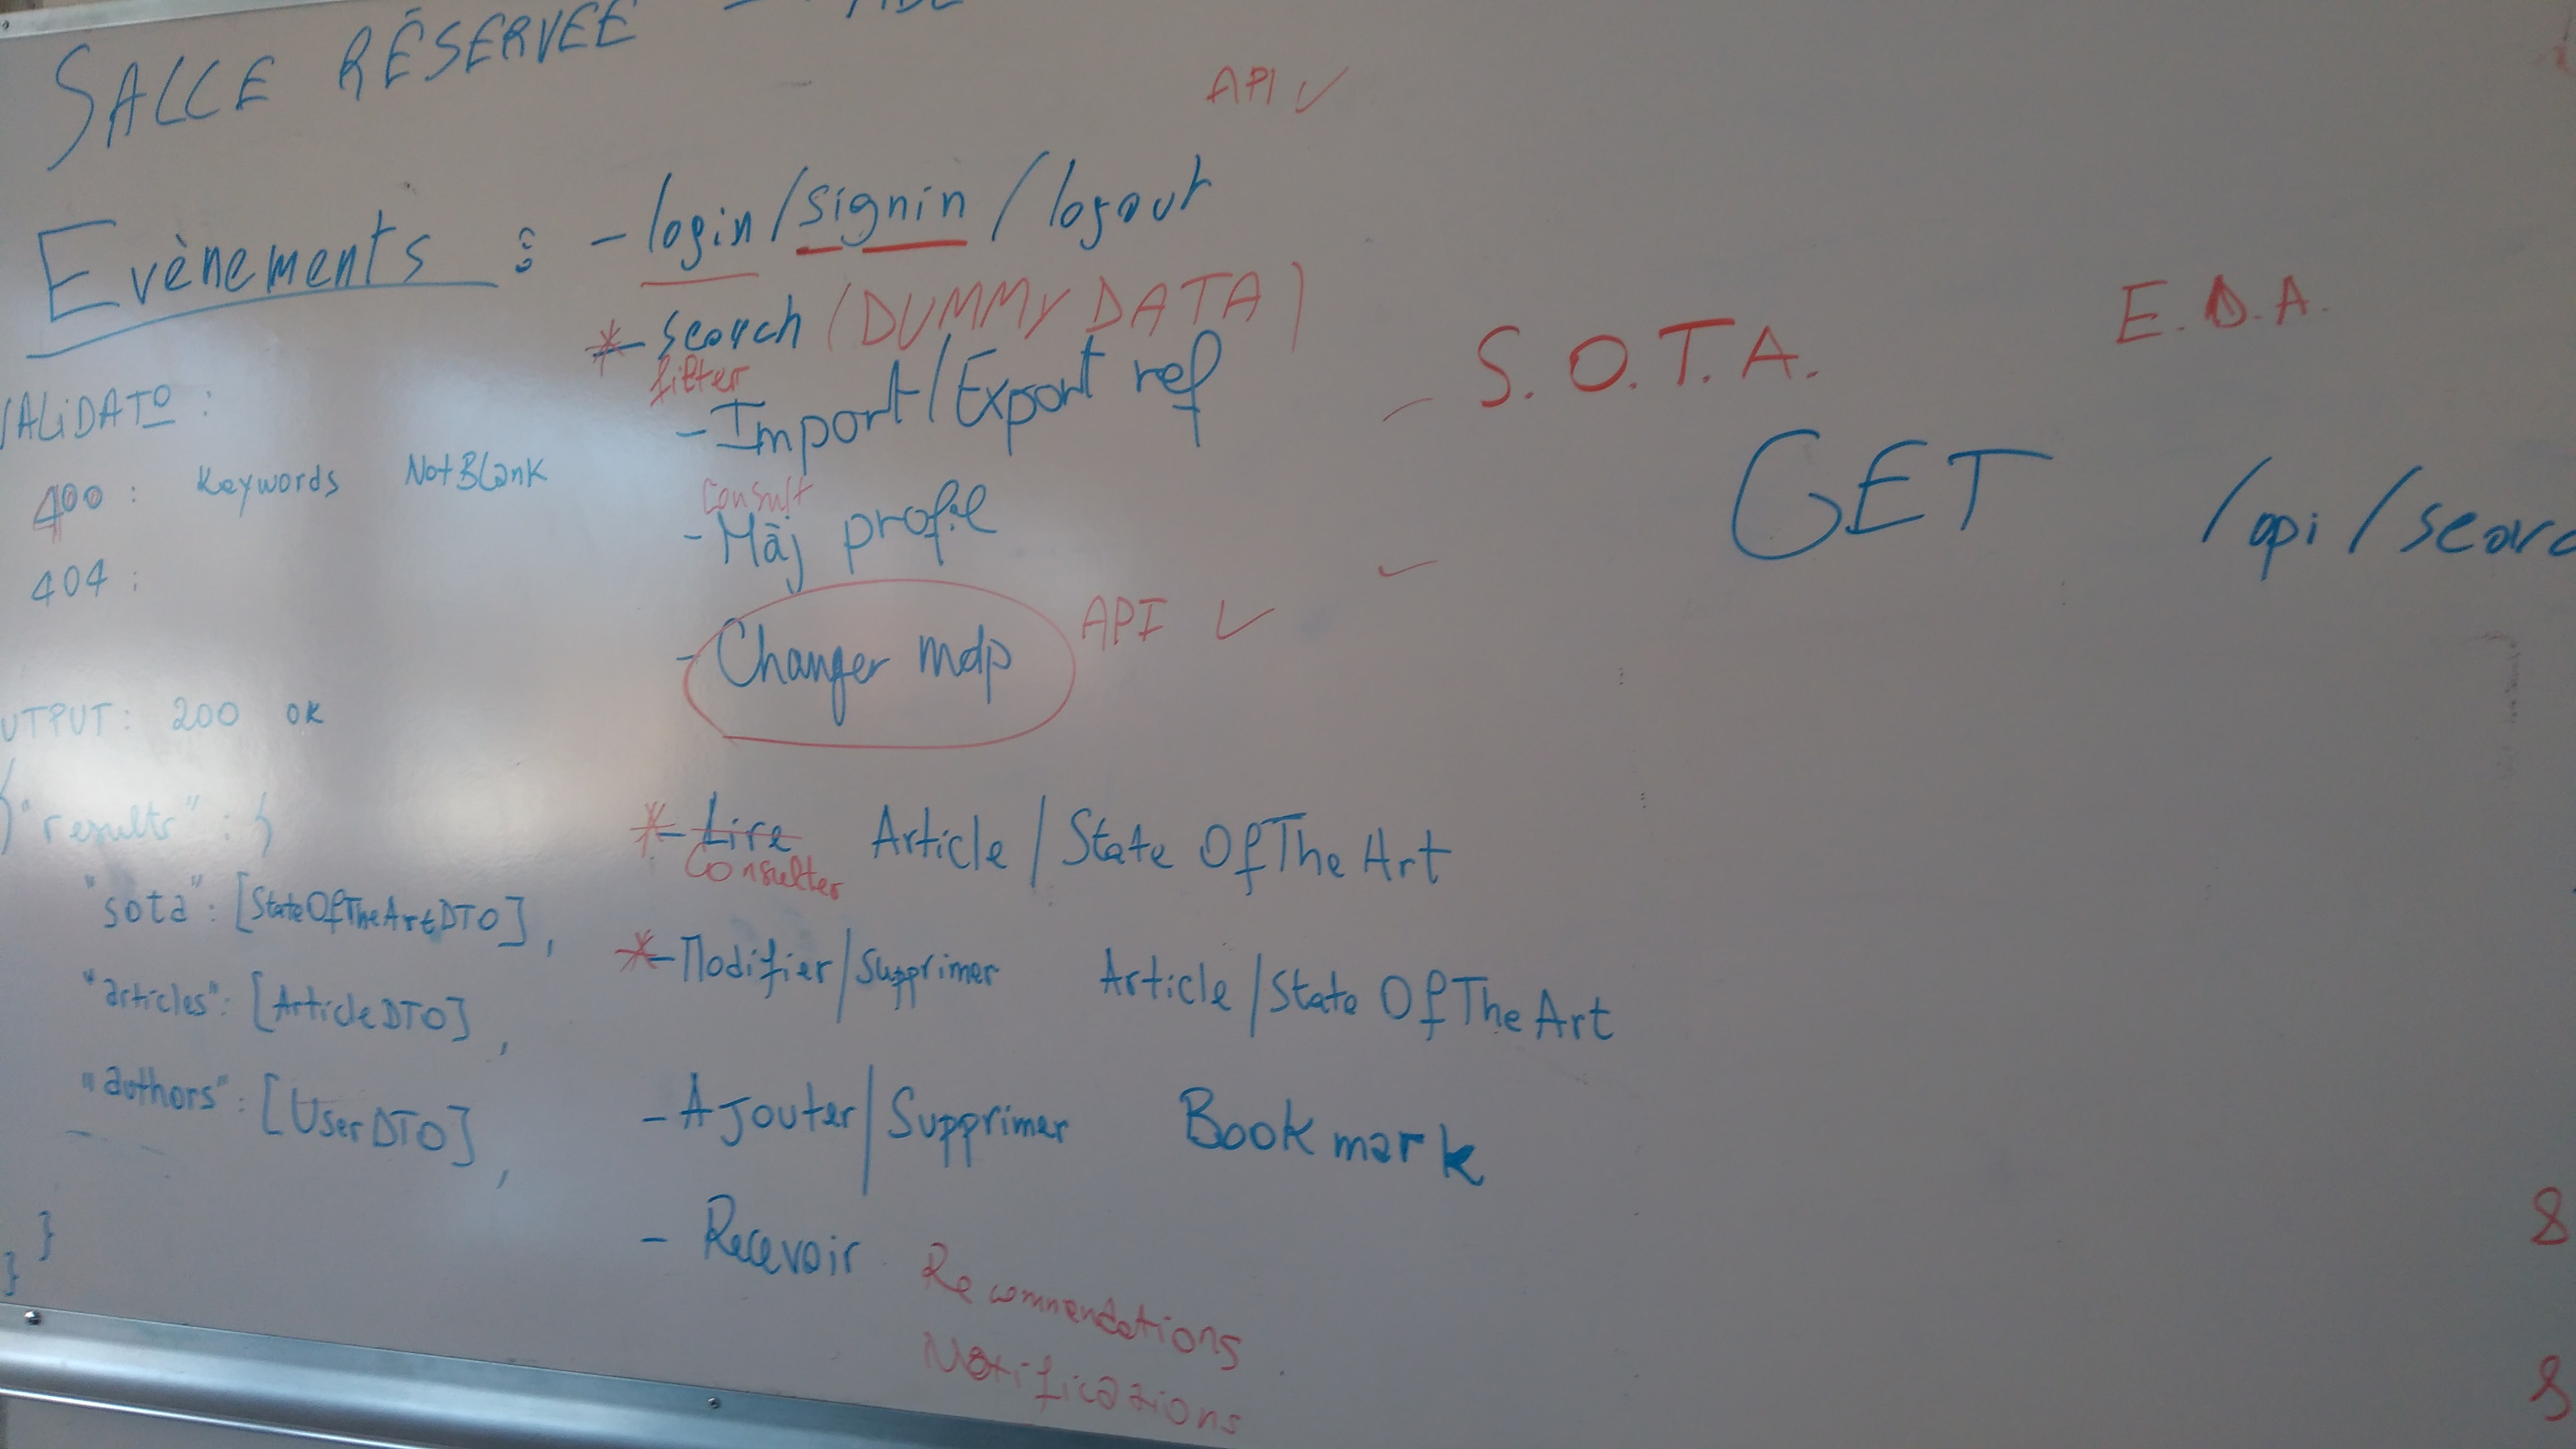
\includegraphics[scale=.08]{images/sprint/exemple-tableau.jpg}
                \captionof{figure}{Aperçu du check-up des fonctionnalités de l'application sur le tableau }
                \label{fig:tableau_todo}
            \end{center}
            
        \newpage
        
        \subsection{Parties prenantes}
            \noindent Les parties prenantes du projet étaient notre client, Antoine CLARINVAL, le professeur en charge du cours d'Ingénierie du Logiciel et Laboratoire, Benoît VANDEROSE, ainsi que deux autres assistants, Adrien VOISIN, responsable des machines virtuelles et Ibtihel TOUKABRI.\\
            Nous avons aussi eu l'honneur de pouvoir parler directement avec certains chercheurs au début du projet pour leur présenter nos idées de base sur la réalisation du projet. Nous avons ainsi reçu leur opinion sur nos idées.

%%%%%%%%%%%%%%%%%%%%%%%%%%%%%%%%%%%%%%%%%%%%%%%%%%%%%%%%%%%%%%%%%%%%
    \newpage
    
    \section{Livrables du projet}
        
        \subsection{Cahier des charges}
            \noindent Nous avons réalisé un cahier des charges afin de nous assurer, d'une part, que nous n'oubliions aucun point et, d'autre part, que notre application serait conforme aux attentes du client. Ce cahier contient l'ensemble des exigences fonctionnelles et non fonctionnelles du projet.
            
        \subsection{Application web}
            \noindent Le projet a été livré sous forme d'une application web déployée, pour que le client puisse la tester et la valider. Le déploiement devait se faire sur une machine virtuelle mise à notre disposition et hébergée sur les serveurs de l'université. Il y a aussi une documentation annexée aux livrables pour expliquer le fonctionnement du site.\\
            Aucun livrable n'a été demandé en cours de projet, nous n'avons dû envoyer l'application qu'à la fin du dernier sprint.
        
        \subsection{Documentation}
            \noindent La documentation est destinée aux utilisateurs. Dans le site, ces derniers ont la possibilité de publier et ajouter des articles ou états de l'art. La documentation sert à expliquer comment faire car cela doit respecter un certain formalisme. La documentation est entre autres là pour rappeler qu'une personne voulant contribuer ou publier doit absolument faire partie d'une institution reconnue et la personne doit s'inscrire au préalable sur le site.

%%%%%%%%%%%%%%%%%%%%%%%%%%%%%%%%%%%%%%%%%%%%%%%%%%%%%%%%%%%%%%%%%%%%%
    \section{Qualité du projet}
        
        \noindent Dès la conception du cahier des charges, nous avons pensé à la qualité du projet en intégrant les exigences de qualité. Nous n'avons pas de plan assurance qualité à part entière mais ce cahier des charges peut en partie servir comme tel, vu qu'il décrit, entre autres, ce que nous avons mis en place pour gérer la qualité de notre application.\\
        Les différents points de qualité dans notre projet sont:
        \begin{itemize}
            \item \textbf{Conformité par rapport aux besoins du client}: le but de ce projet était de créer une application web qui permet de créer, visualiser et trouver facilement des états de l'art. Notre application permet bien de réaliser ces différentes tâches.
            
            \item \textbf{Fiabilité}: l'application fonctionne correctement avec un haut taux de fiabilité. Elle ne plante pas et toutes les fonctionnalités demandées et prévues à la base sont présentes et fonctionnelles.
            
            \item \textbf{Efficacité}: l'application se charge et réagit rapidement, pour autant que la connexion internet de l'utilisateur soit correcte (convenable ou optimale). L'application demande une quantité de mémoire relativement importante mais cela n'affecte pas les performances de l'application.
            
            \item \textbf{Intégrité}: l'inscription sur la plate-forme requiert un mot de passe fort composé de chiffres et lettres minuscules et majuscules. L'utilisation de l'API requiert un token d'accès, seulement valable après authentification.
            
            \item \textbf{Ergonomie}: l'application est facile d'utilisation, tout au plus 4 clics sont requis pour réaliser une action. La documentation est là pour aider ceux qui en ont besoin mais 95\% des utilisateurs n'en auront pas besoin.
            
            \item \textbf{Maintenabilité}: le code produit respecte plusieurs principes appris en cours d'ingénierie d'architecture logicielle (IALTEM).
            \item \textbf{Souplesse}: chaque partie de l'application a été écrite de manière indépendante. Ainsi, l'évolution de l'application peut se faire sans violer les spécifications définies. Par exemple, on pourrait envisager de remplacer l'application par un application mobile Android, il suffirait simplement de modifier le front-end sans toucher au back-end.
            \item Testabilité:
            \item Portabilité: l'application est utilisable sur n'importe quelle machine connectée à internet, pour autant qu'elle dispose d'un navigateur à jour.
            \item Réutilisabilité: l'application est faites de nombreux composants, réutilisés à plusieurs endroits dans le code et réutilisables dans d'autres logiciels.
        \end{itemize}
        
        \noindent Ces décisions ont été prises sans le client mais nous avons tenu compte de ses remarques lors des sprint reviews et apporté les modifications demandées.\\
        Les seuls critères d'acceptation étaient que le livrable de l'application devait être un lien vers celle-ci, mise en production, utilisable et testable.
        
    
%%%%%%%%%%%%%%%%%%%%%%%%%%%%%%%%%%%%%%%%%%%%%%%%%%%%%%%%%%%%%%%%%%%%%

    \newpage

    \section{Gestion des risques}
    \noindent Nous avons identifié deux risques en début de projet et ceux-ci ont bien été gérés dès le départ. Nous avons cependant rencontré un troisième risque en cours de projet. 
    
    \begin{enumerate}
        \item  Le premier risque identifié était le partage du code entre nous. Nous nous y sommes confrontés dès le début du projet. Pour gérer ce problème, nous avons choisi d'utiliser Github, qui permet de  centraliser le code et de gérer les conflits de différence entre les versions de code de chacun. Pour le placer au niveau de la matrice de probabilité de risque, il revenait à 70\% de probabilité et 0,56 niveau impact du risque. \\
        \item Un autre risque était l'utilisation de technologies différentes. Afin d'éviter que chaque personne n'utilise une technologie différente, il a fallu se mettre d'accord sur les technologies, utilisée à la fois en back-end et en front-end. Nous avons géré ce risque en commençant par comparer les technologies et libraires à notre disposition en tenant compte des contraintes.
        Ensuite, avant de nous lancer dans le développement, chaque groupe a du apprendre les bases des technologies à utiliser pour sa partie de l'application.\\
        Enfin, pour combler les différentes lacunes ou ..., on a réalisé du pair programming.
        Concrètement, à chaque fois qu'un membre du groupe ne pouvait pas réaliser sa tâche ou était dans l'impossibilité de la faire, un autre membre ayant déjà réalisé sa tâche ou ayant un peu plus d'expérience venait épauler les autres.
        \newline
        \item Un risque lié au produit est les navigateurs. Les visualisations proposées dans l'application étaient dépendantes du \textit{navigateur} et de sa version de \textit{Javascript}. Il était fort possible qu'avec certains navigateurs, l'affichage de la visualisation ne soit pas disponible ou ne soit pas correct. Pour réduire l'impact, nous avons affiché l'application sur plusieurs navigateurs et choisi le navigateur le plus optimal pour l'affichage des visualisations. Nous avons conseillé ce navigateur pour avoir la meilleure expérience utilisateur.
        \newline
    \end{enumerate}
    

        
    \textit{IN PROGRESS ...}
        
    
%%%%%%%%%%%%%%%%%%%%%%%%%%%%%%%%%%%%%%%%%%%%%%%%%%%%%%%%%%%%%%%%%%%%%
    
    \newpage
    
    \section{Planification du projet}
        \subsection{Scope Management}
        \noindent Nous avons commencé le projet par une phase de conception et d'analyse. Une fois l'analyse faite à notre niveau et validée par le client, avec certaines remarques, nous avons commencé par l'apprentissage des outils et technologies à utiliser durant le développement. Nous sommes ensuite passés à l'installation de tous les outils et librairies nécessaires pour le bon déroulement du projet. Une fois la mise en place terminée, la phase de développement a commencé.\\
        La plus grosse partie au lancement du projet était le back-end. L'équipe front-end s'est aussi lancée de son côté dans la réalisation de ses tâches. La connexion entre le back-end et le front-end n'a cependant été faite qu'une fois le back-end entièrement fonctionnel, pour permettre d'avancer sur le reste sans devoir attendre.
        Ci-dessous se trouve une brève description de nos \textit{sprints} : 

            \subsubsection{Sprint 1}
                \noindent Le premier sprint était centré sur la découverte de  Jira, la mise en commun et au propre de nos idées via des post-it en classification Must-have et Nice-to-have. 
                
                                
                 \begin{center}                       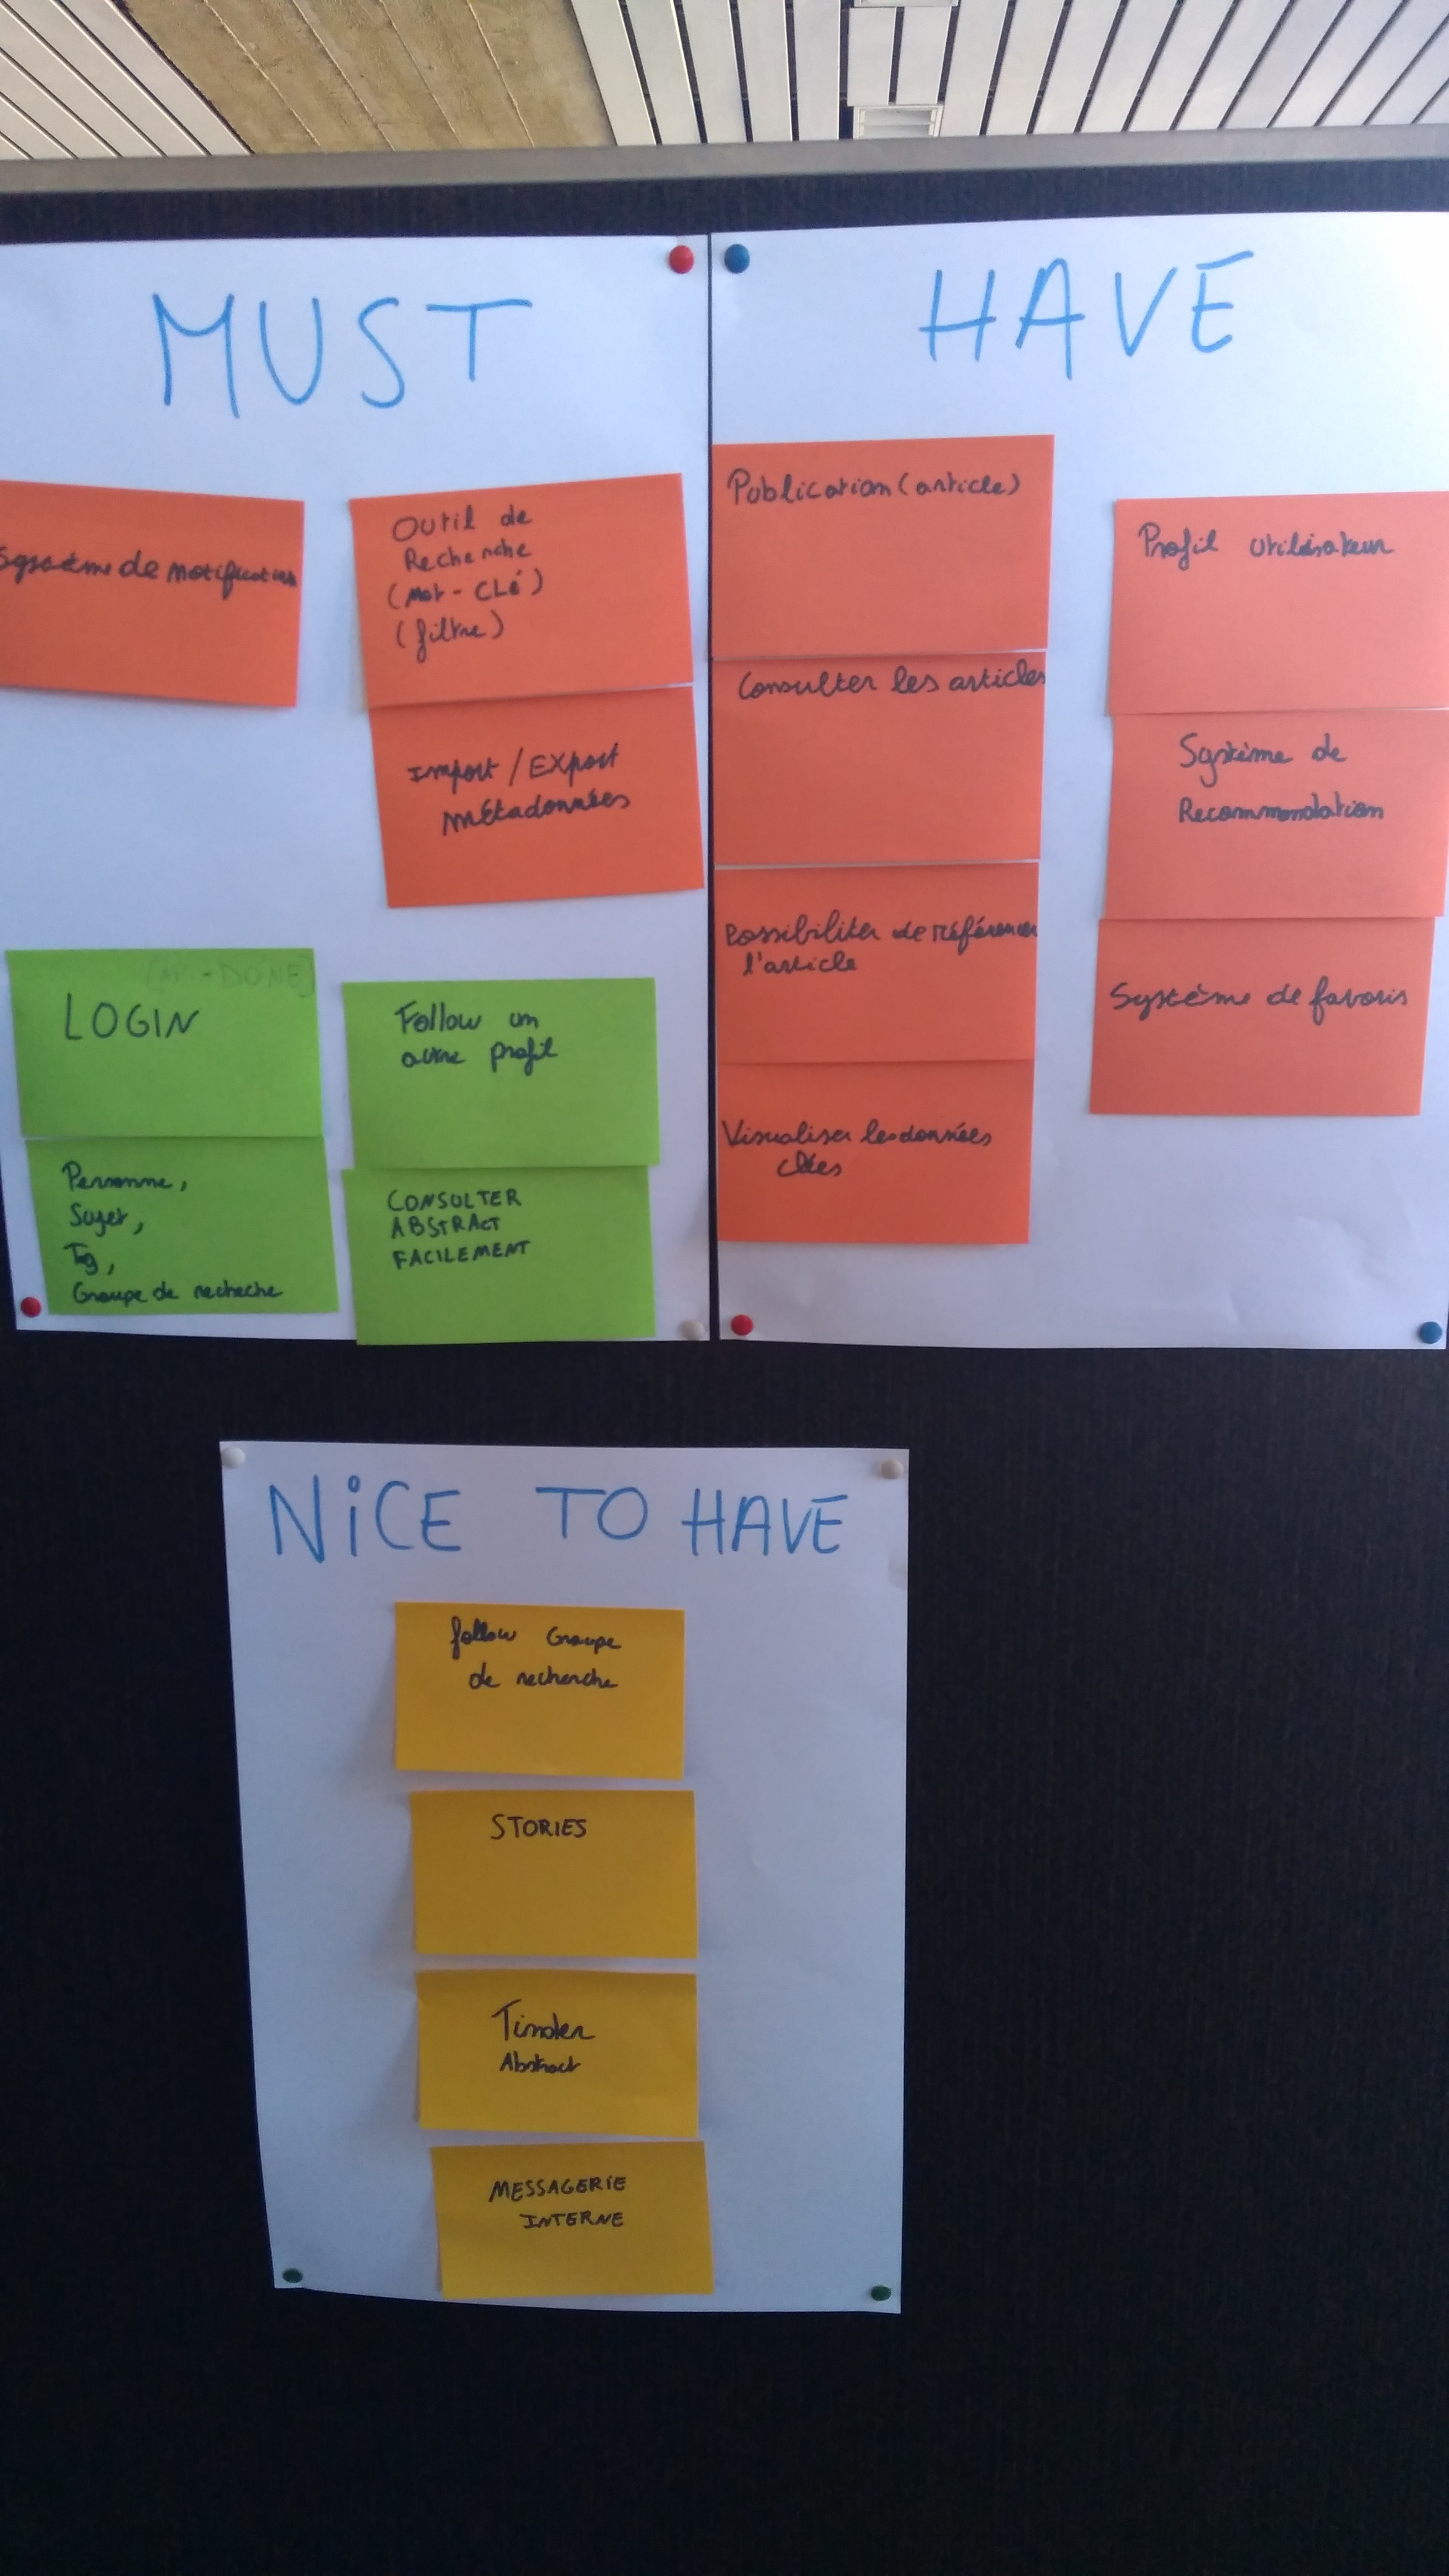
\includegraphics[scale=.07]{images/sprint/must-nice-have.jpg}
                    \captionof{figure}{Sprint 1: Nice to and must have board}
                    \label{fig:sprint1_graph}
                \end{center}
                
                \newpage
                
                \noindent Nous avons réalisé un mini design thinking sur les interfaces de l'application via des prototypes papier. Après concertation et choix des meilleurs modèles et composants à concevoir, nous avons transformé nos prototypes en wireframe via une application en ligne.
                
                \begin{center}
                    
                    \begin{figure}[h]       
                        \fbox{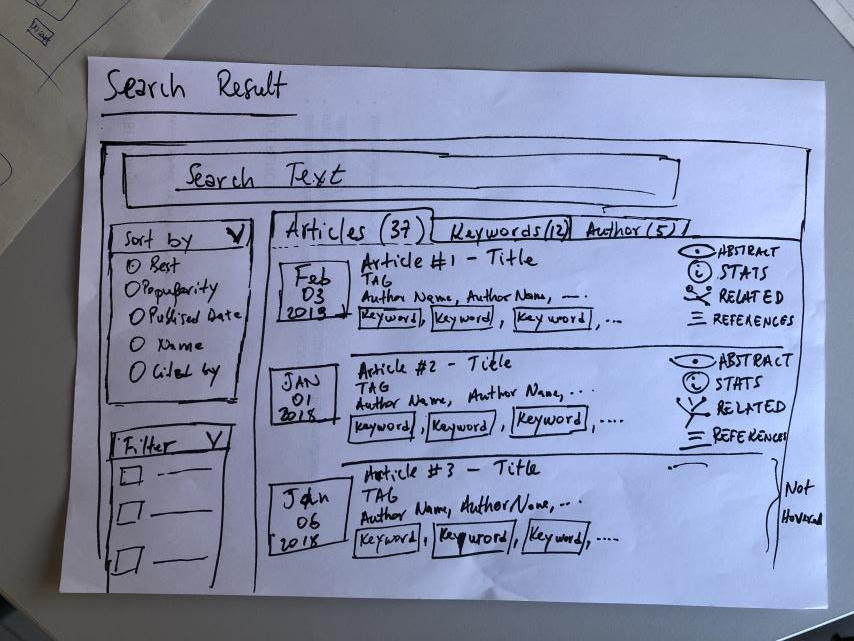
\includegraphics[scale=.27]{images/protos/proto-papier.jpg}}   
                        \hfill                        \fbox{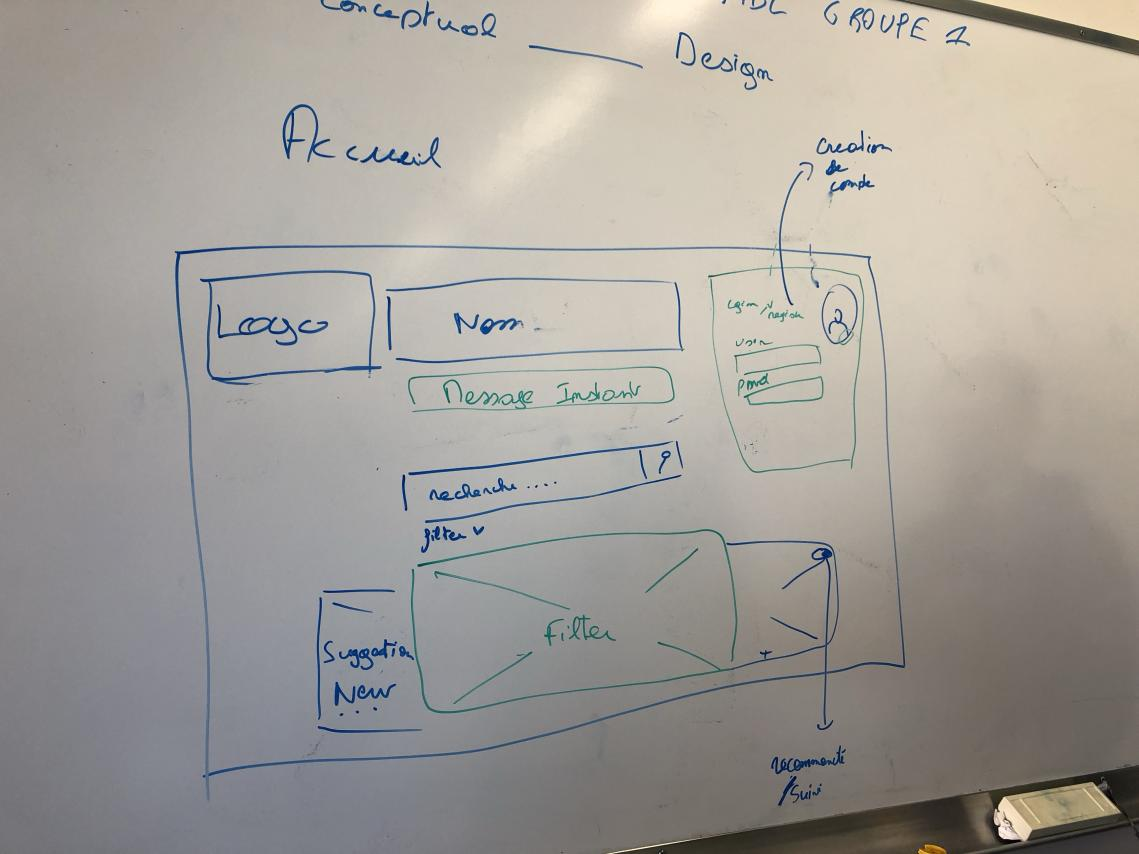
\includegraphics[scale=.2]{images/protos/proto-tableau-0.jpg}}
                        \hfill                        \fbox{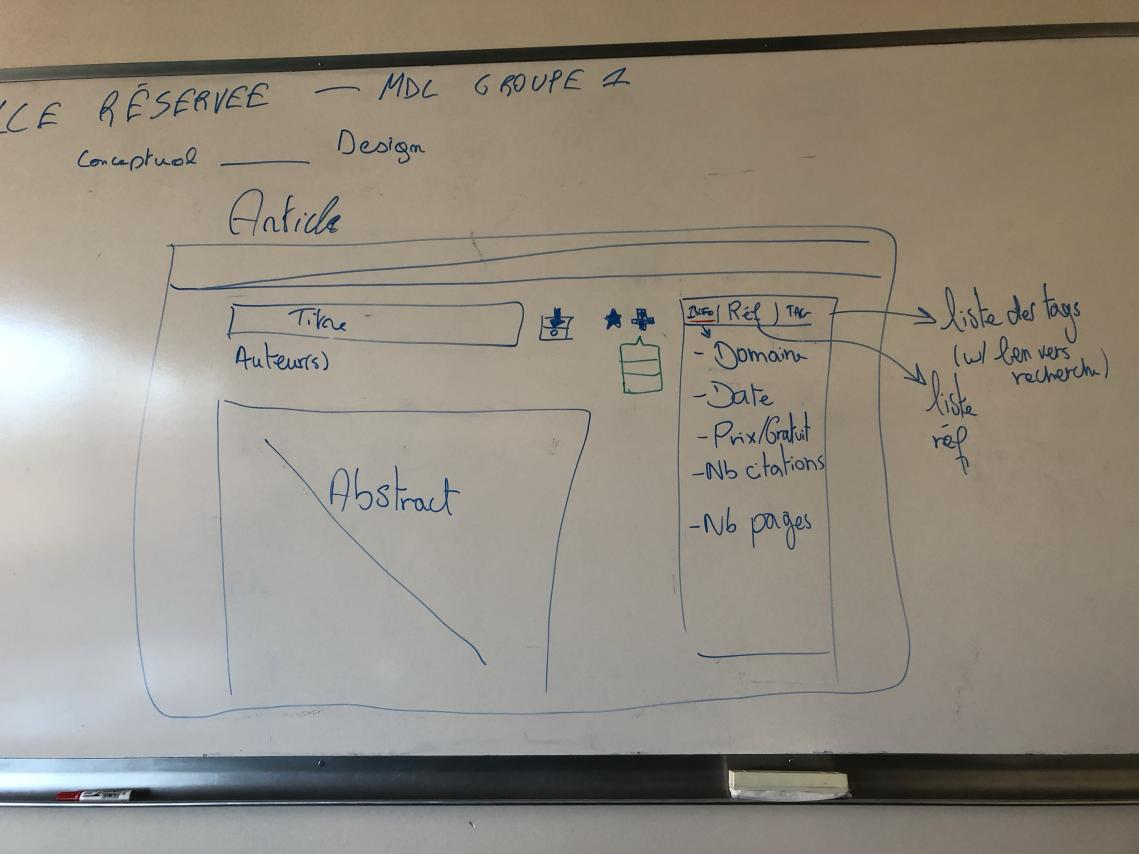
\includegraphics[scale=.2]{images/protos/proto-tableau-1.jpg}}
                        \hfill
                        \fbox{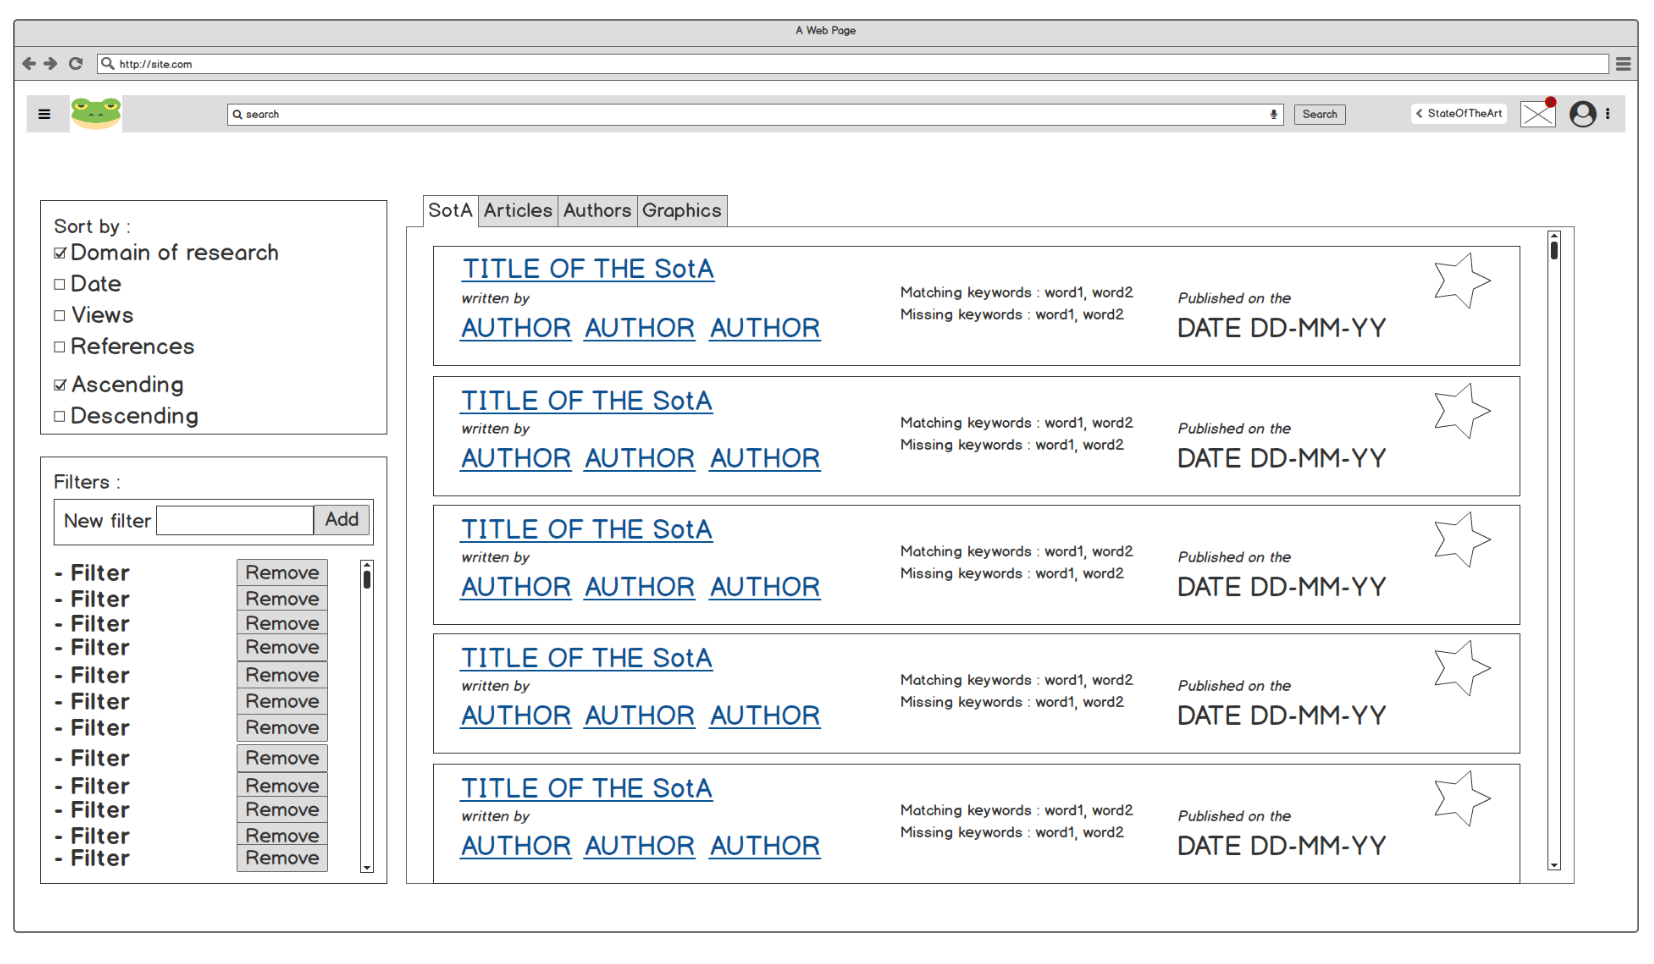
\includegraphics[scale=.165]{images/protos/wireframe.png}}
                        \caption{Sprint 1: Aperçus de prototypes et wireframes}
                        \label{fig:sprint1_protos}
                    \end{figure}
            \end{center}   
                
                \newpage
                
                \noindent Enfin, nous avons créé des personna (utilisateurs types) pour enrichir nos user stories et fonctionnalités.
                
                 \begin{center}
                    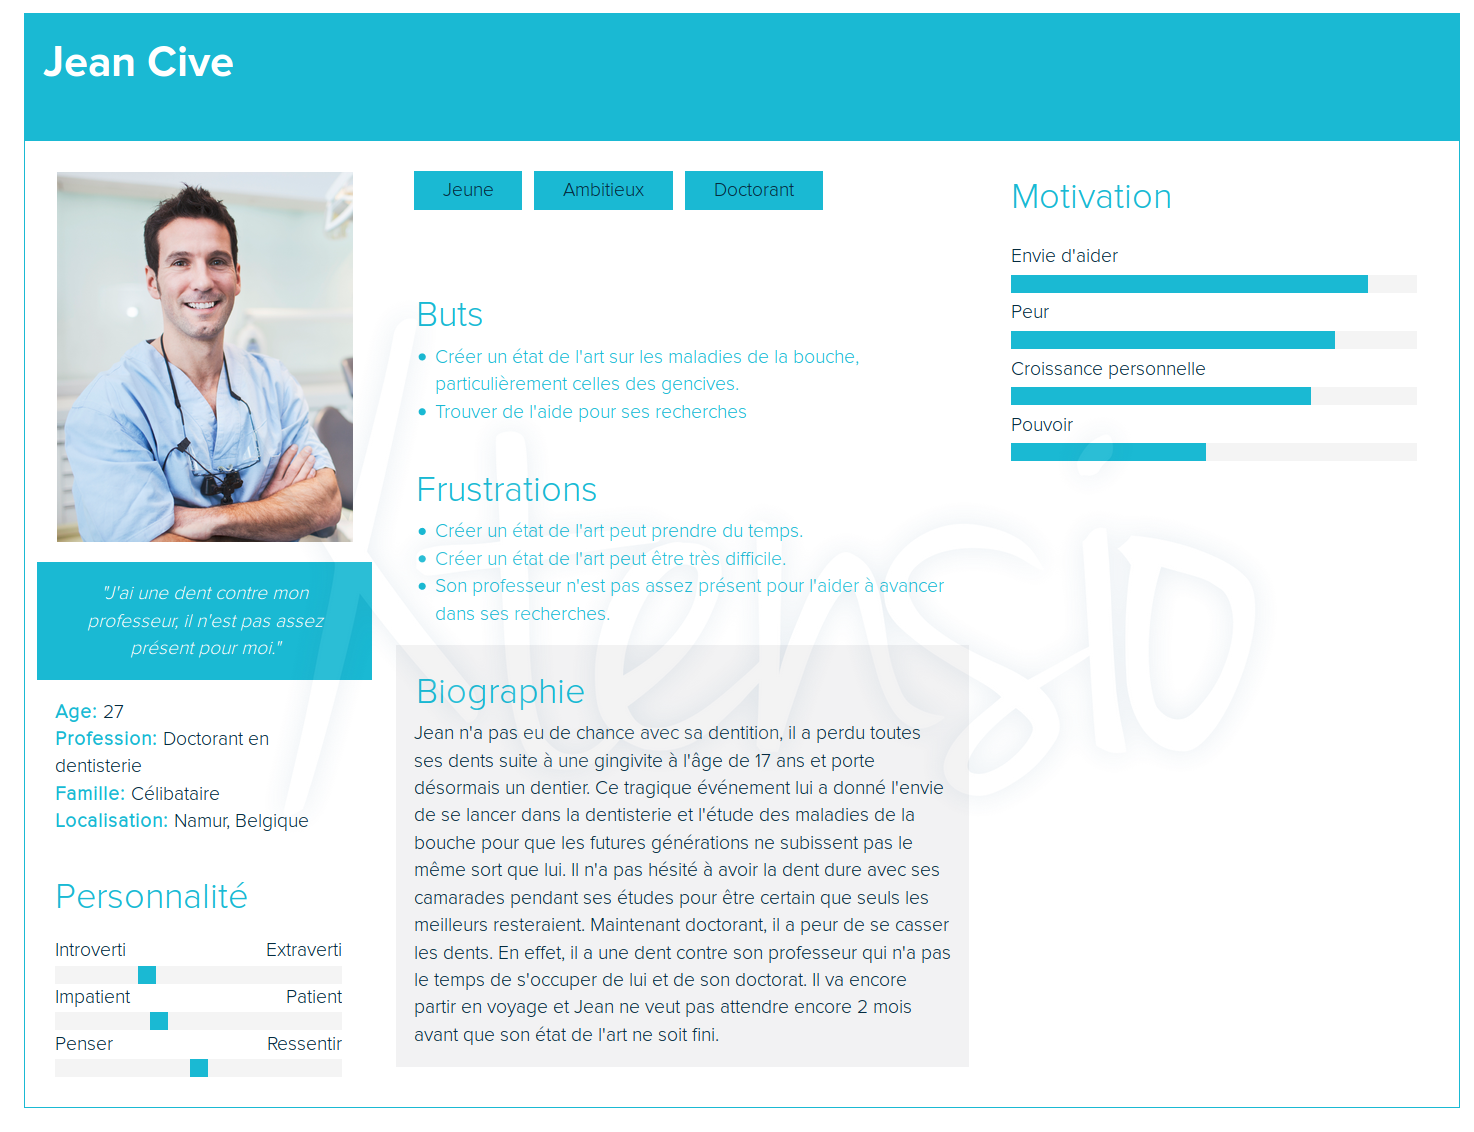
\includegraphics[scale=.2]{images/sprint/personna-jean-cive.png}
                    \captionof{figure}{Sprint 1: Personna principal - Jean Cive}%
                    \label{fig:sprint1_personna}

                    \begin{figure}[!htb]
                        \minipage{0.48\textwidth}
                            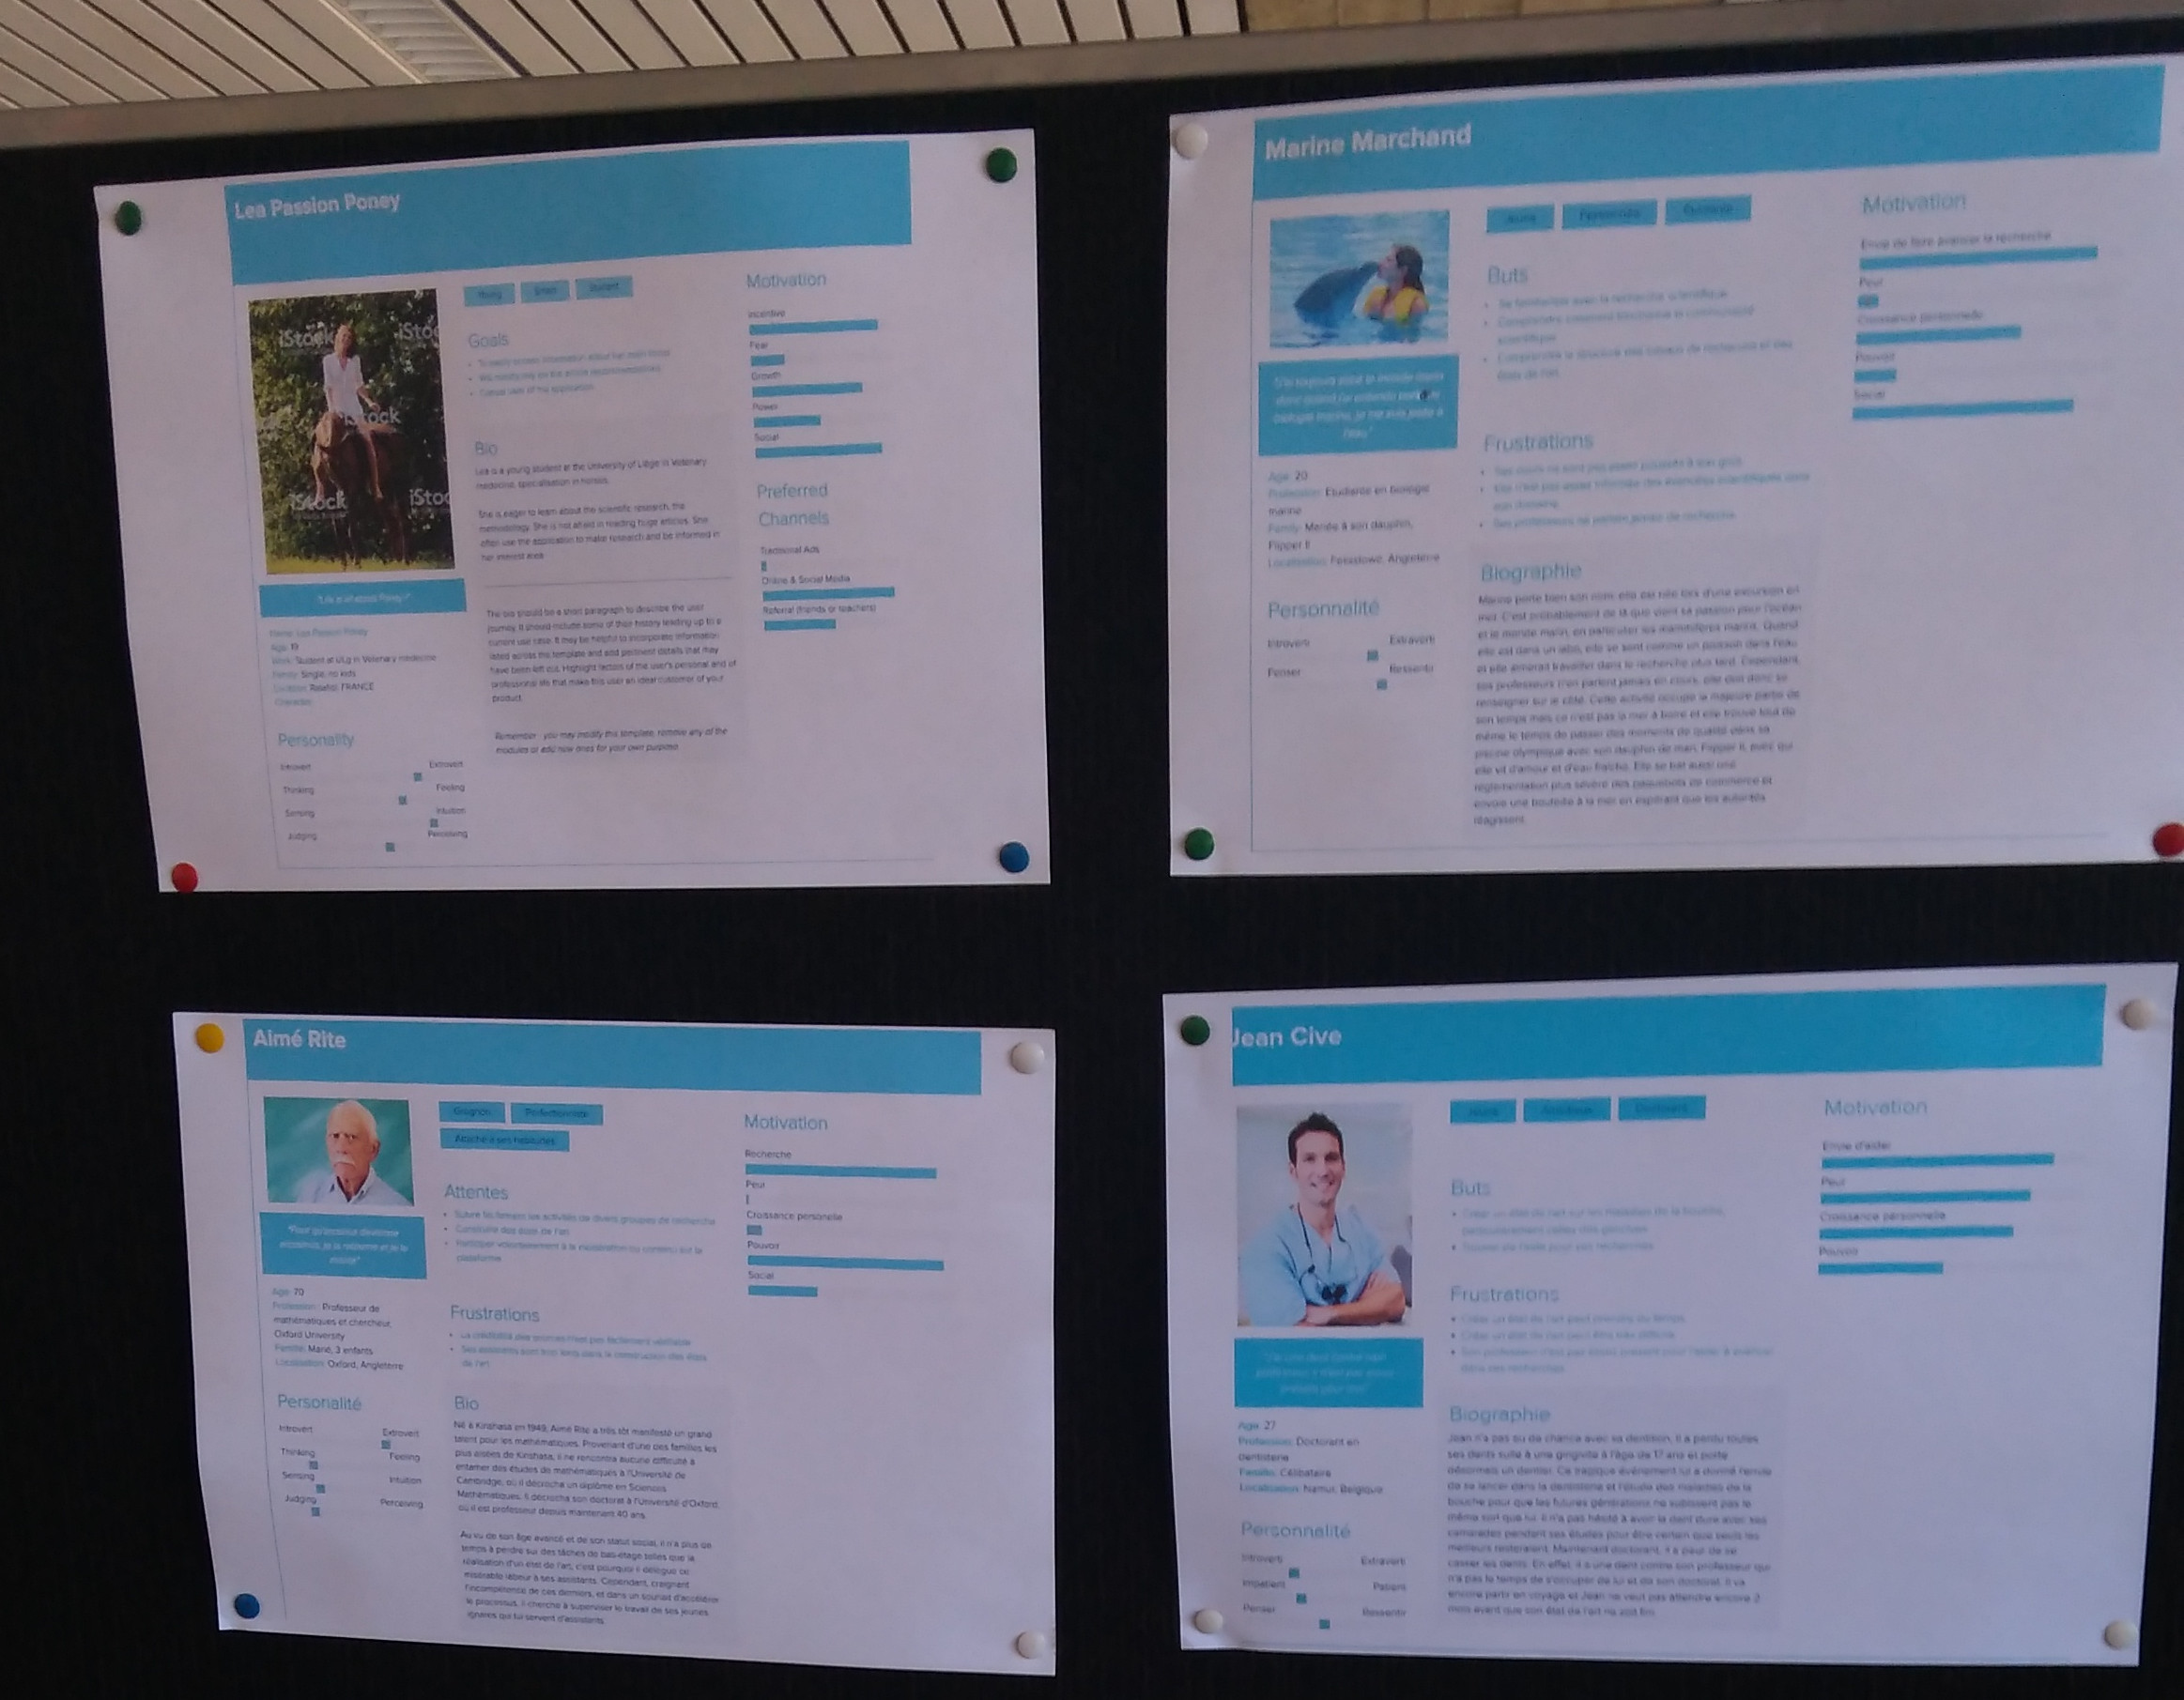
\includegraphics[width=\linewidth]{images/sprint/personas.jpg}
                            \caption{Personnas board}\label{fig:board_user_personnas}
                        \endminipage
                        \hfill
                        \minipage{0.48\textwidth}%
                            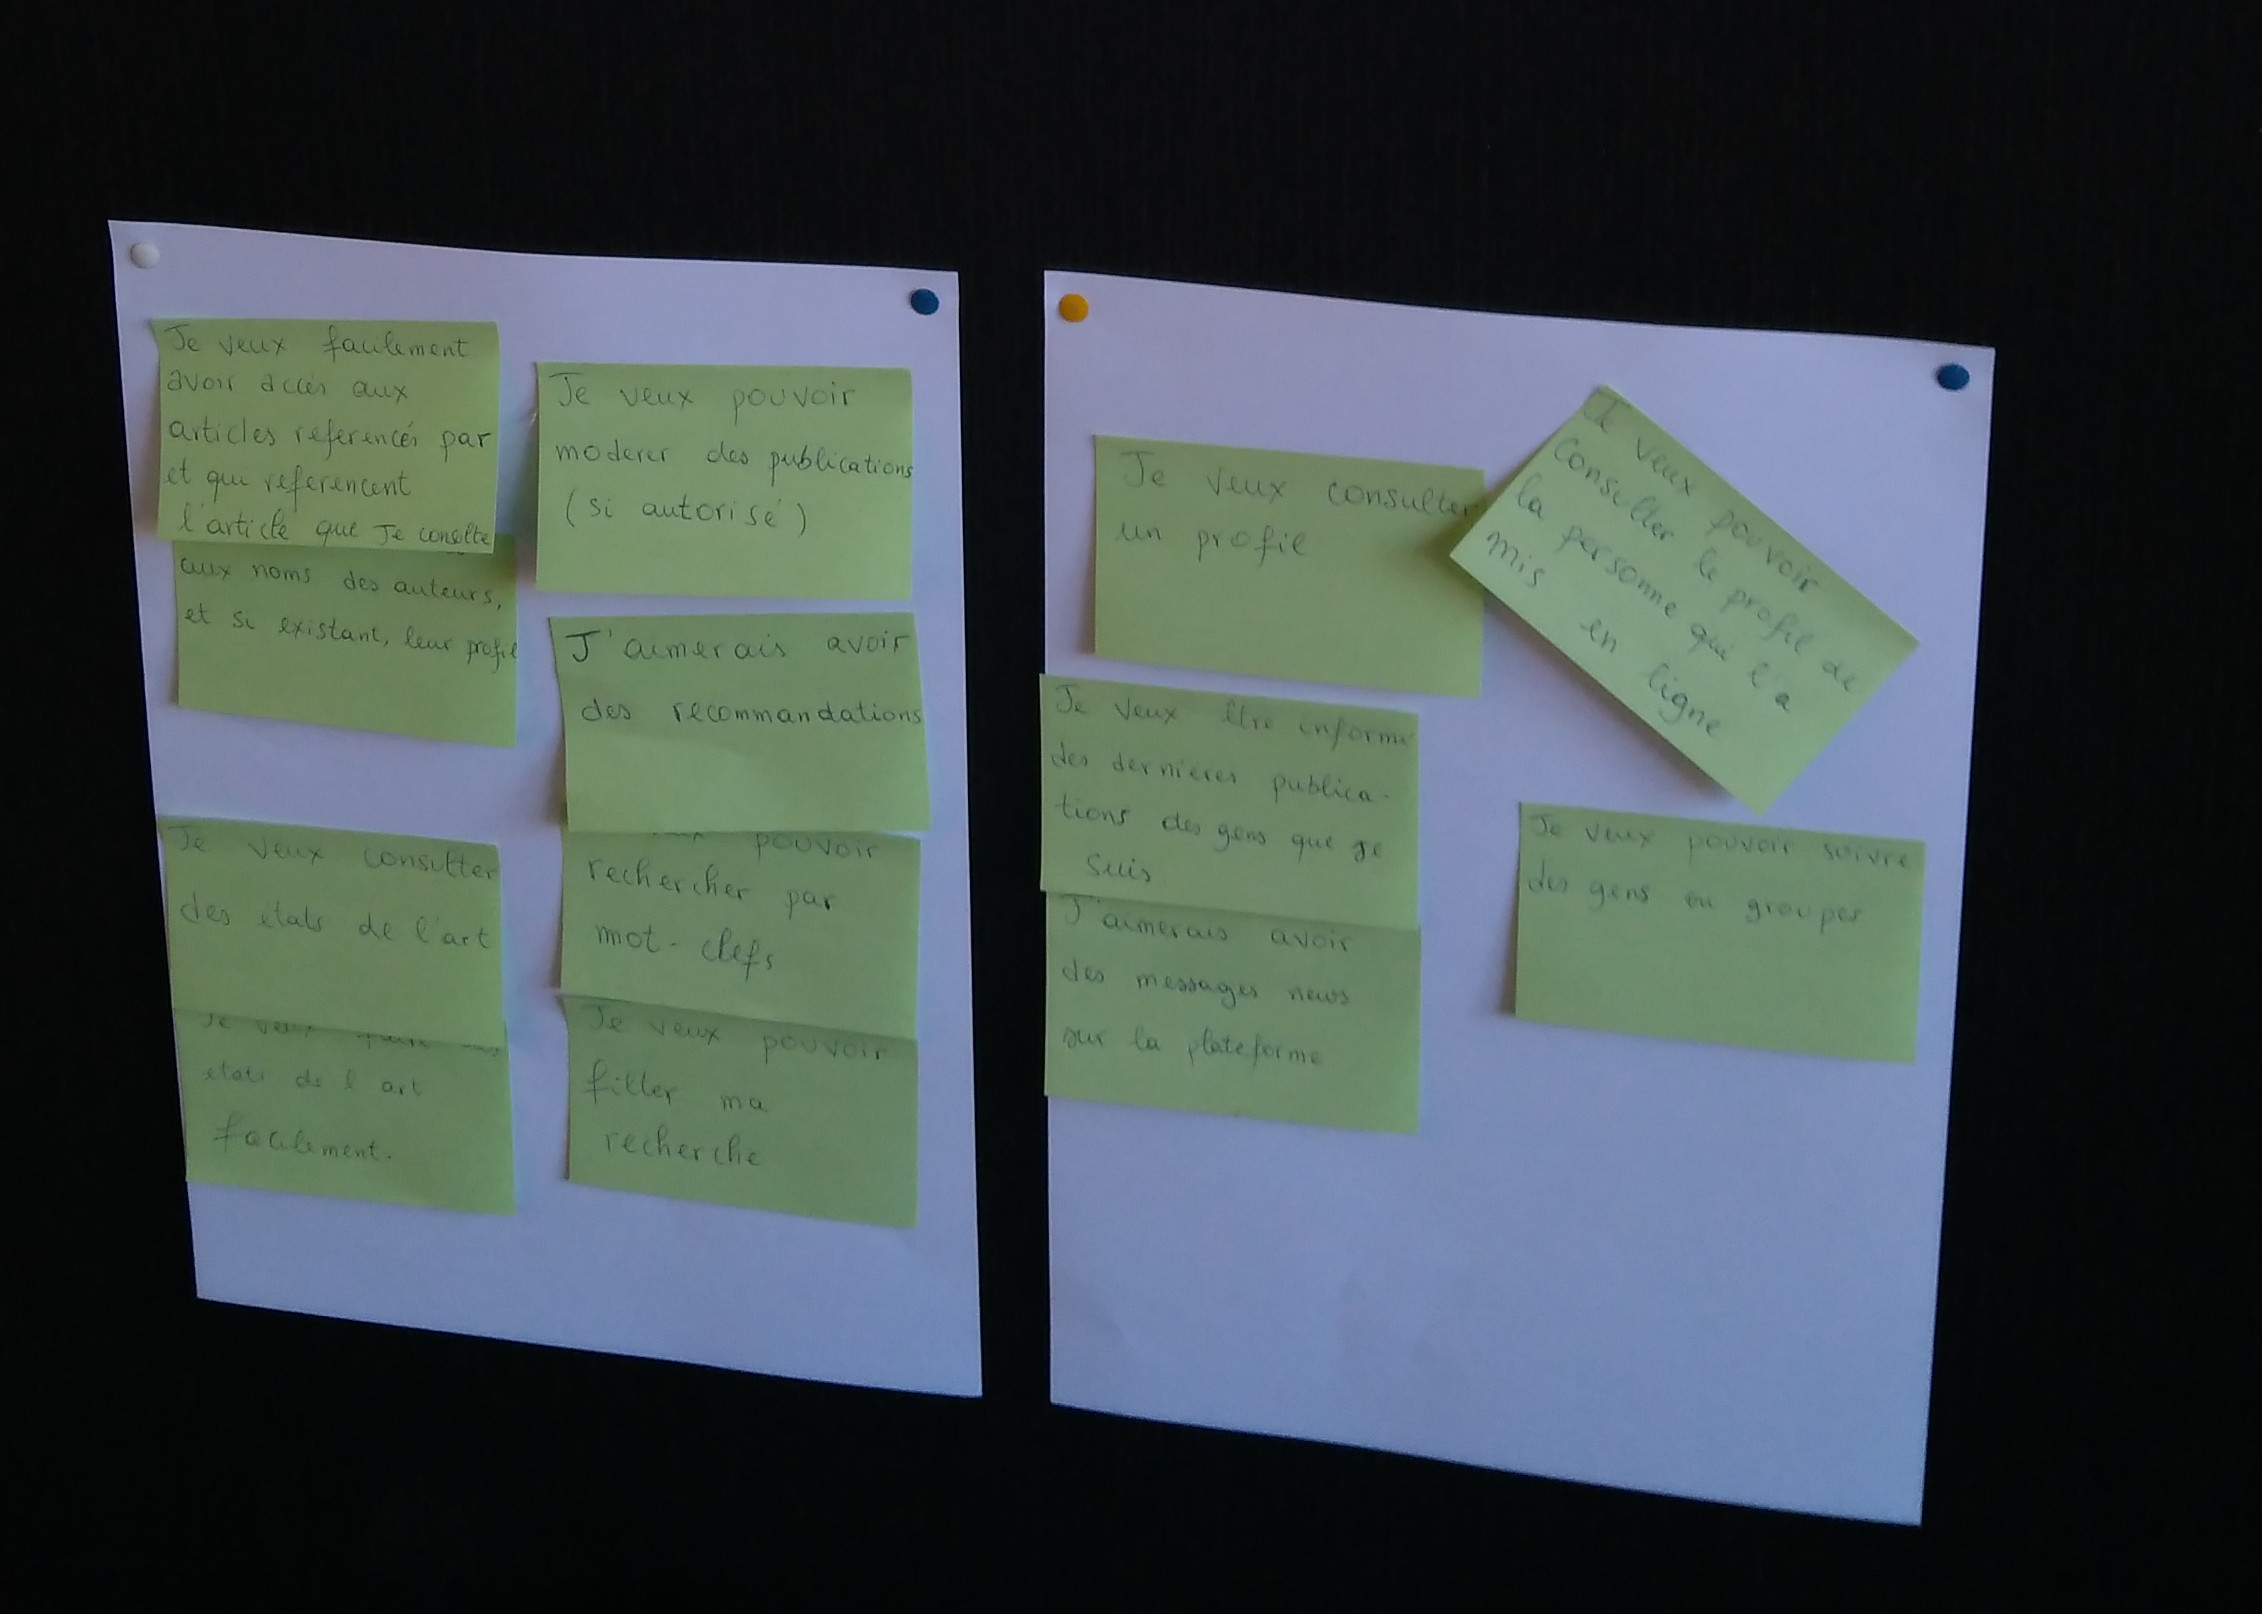
\includegraphics[width=\linewidth]{images/sprint/user-stories.jpg}
                            \caption{User stories}\label{fig:board_user_stories}
                        \endminipage
                    \end{figure}
            \end{center}                

                
                 \begin{center}
                    %%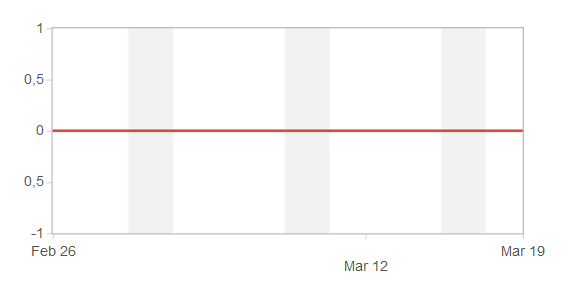
\includegraphics[scale=1]{images/graph/sprint1.png}\\
                    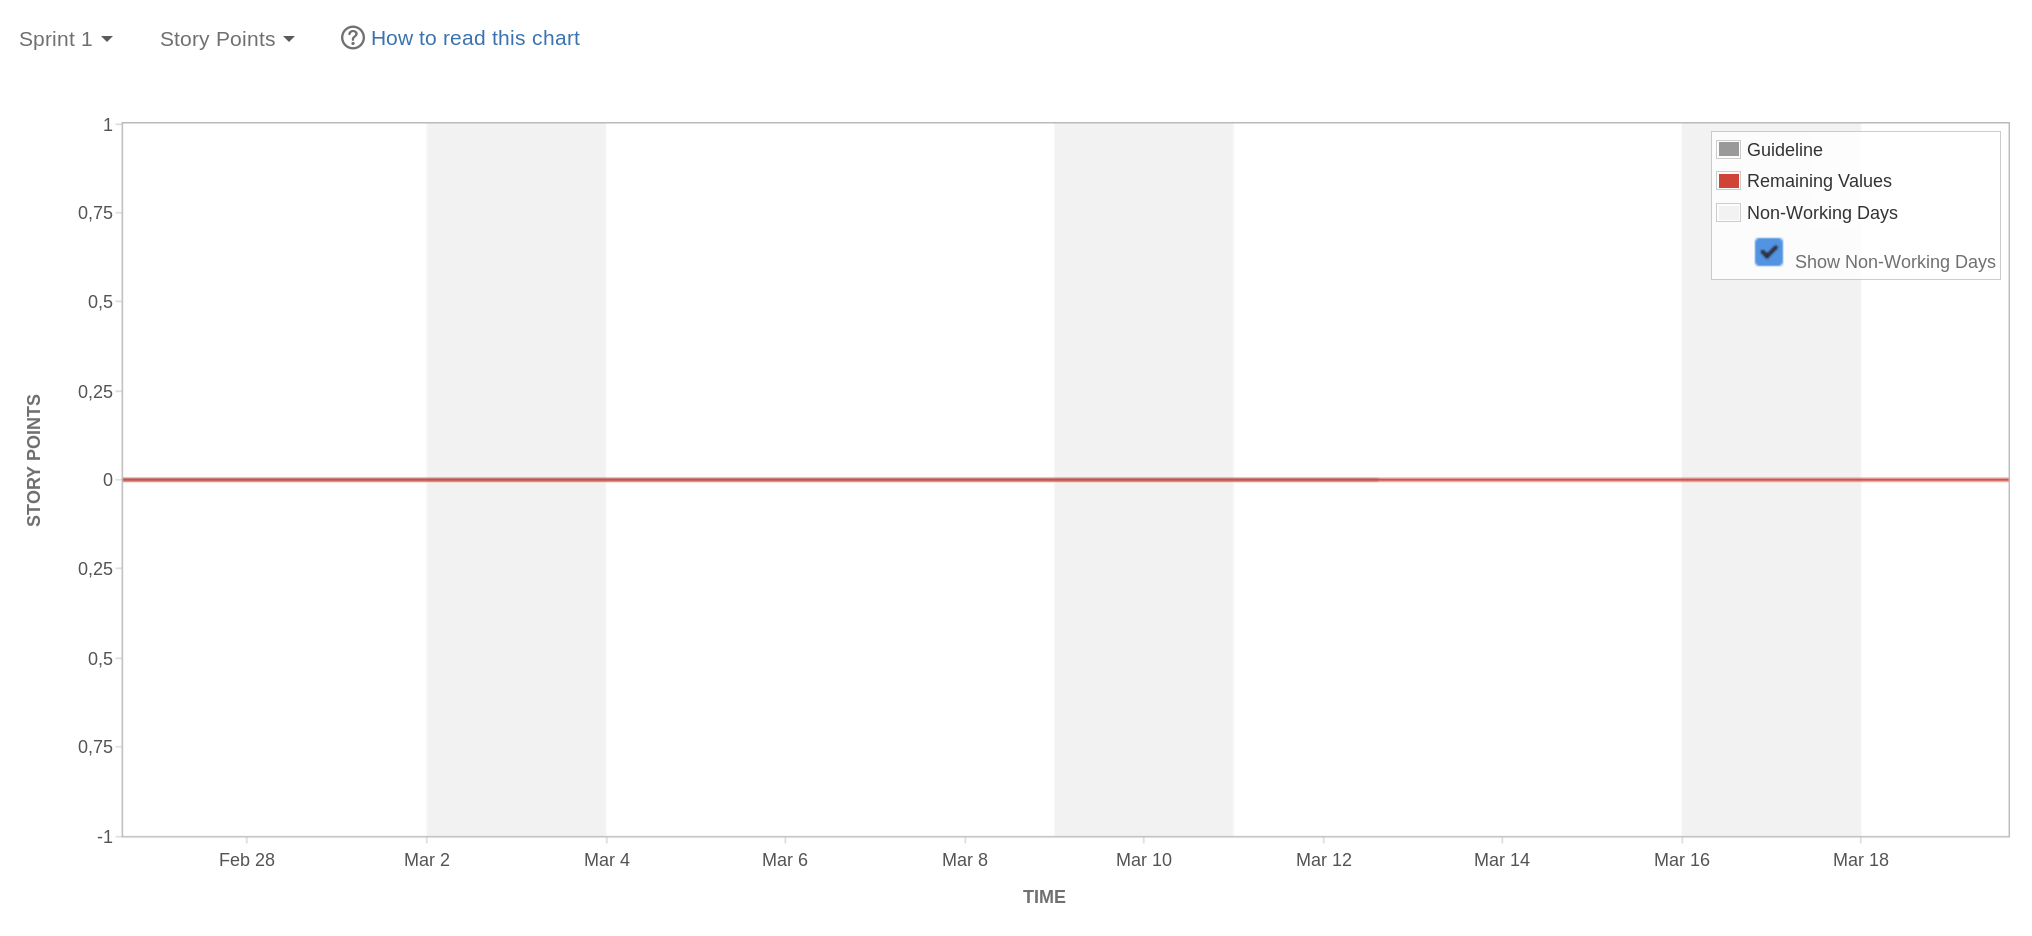
\includegraphics[scale=.25]{images/graph-new/sprint1.png}
                    \captionof{figure}{Sprint 1: Burndown chart}%
                    \label{fig:sprint1_graph}
                \end{center}
                Comme le montre ce premier burndown chart \ref{fig:sprint1_graph}, nous avions oublié d'estimer nos tâches et donc celui reste toujours à 0.
                
                
            \subsubsection{Sprint 2}
                \noindent Durant ce deuxième sprint, nous avions peaufiné les précédents wireframes et entamé ceux concernant les visualisations disponibles dans l'application web. Nous avons appris de notre précédente erreur, ainsi, pour l'estimation des tâches actuelles et futures, nous avons utilisé une échelle de valeur suivant les chiffres de Fibonacci: 1, 2, 3, 5, 8. Plus le chiffre est grand, plus il faudra d'efforts pour accomplir la tâche. Nous nous sommes réparti les tâches de manière à ce que chaque membre de l'équipe ait une charge de travail égale. Le SM distribuait les tâches pour que chaque personne ait une charge de travail égale à 10 points (2 tâches à 5 points, 3 tâches à 3 points et une à 1 point,...).
                \newline
                Nous nous sommes rendus compte que l'on avait oublié le sprint retrospective au sprint précédent. Nous l'avons donc fait à la fin de ce sprint review. 
                Nous avons utilisé le tableau du local et de post-it de différentes couleurs. Nous avons établi 4 catégories \textit{K.I.S.S.} (Keep, Improve, Start doing, Stop doing) et chacun devait se servir des post-it pour suggérer des activités ou idées pour améliorer le prochain sprint.


                \begin{center}                               
                    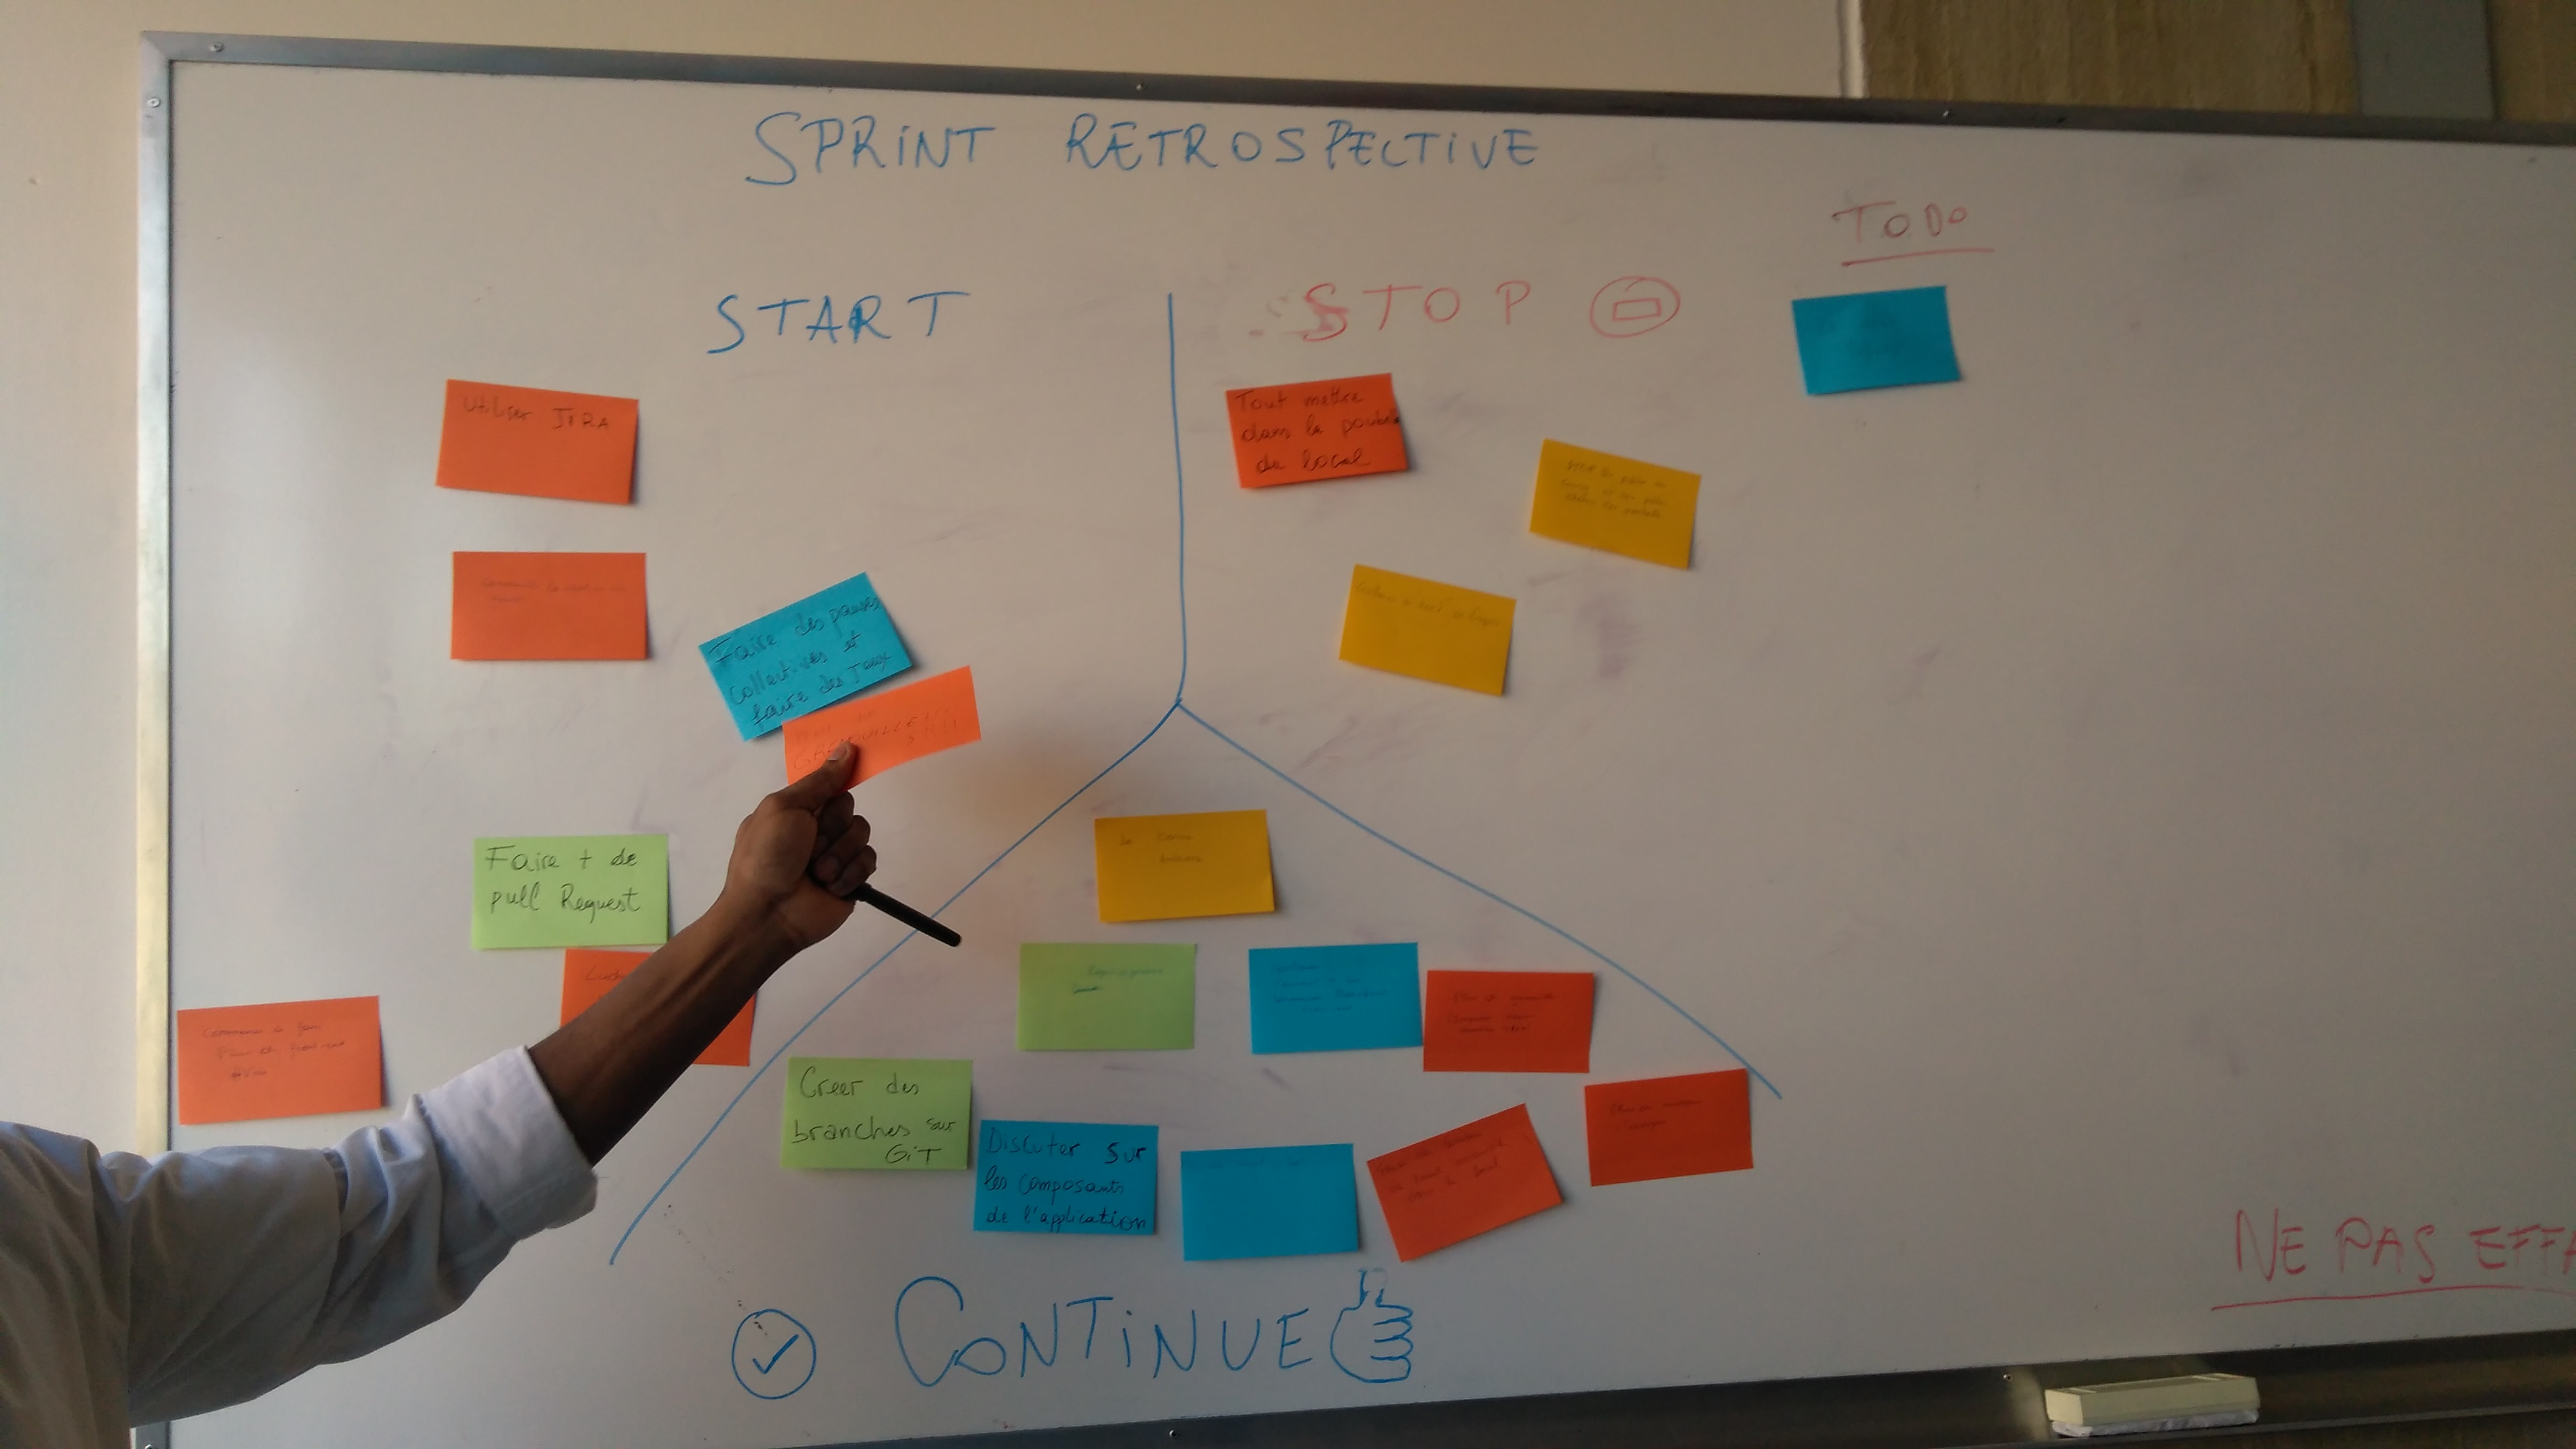
\includegraphics[scale=.1]{images/sprint/sprint-retro.jpg}
                    \captionof{figure}{Sprint 1: Sprint rétrospective}
                    \label{fig:sprint1_graph}
                \end{center}

                \begin{center}
                    %%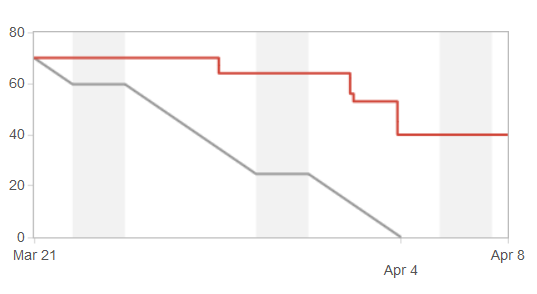
\includegraphics[scale=1]{images/graph/sprint2.png}
                    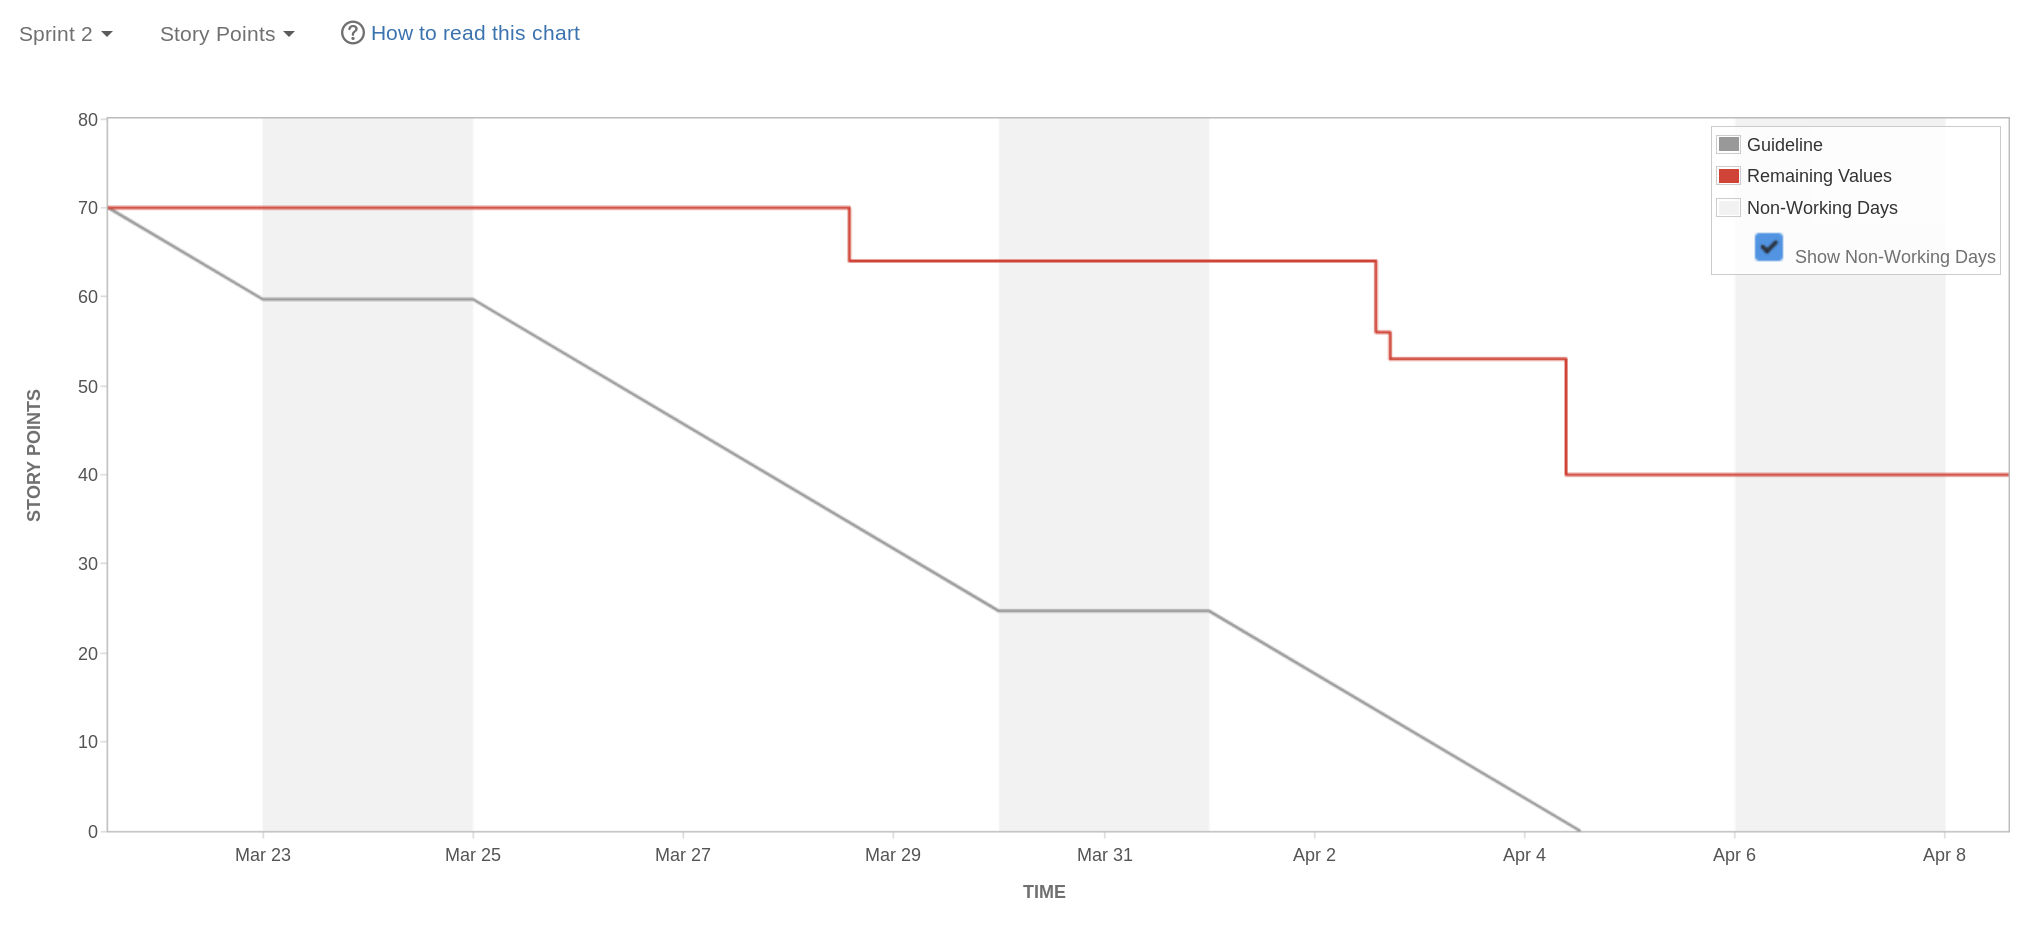
\includegraphics[scale=.25]{images/graph-new/sprint2.png}
                    \captionof{figure}{Sprint 2 - Burndown chart}
                    \label{fig:sprint2_graph}
                \end{center}

                \noindent On remarque, cette fois-ci, un grand de retard entre ce qui a été prévu et le travail réellement achevé. Ce retard est dû à de mauvaises estimations. Nous n'avions en effet pas tenu compte ni de l'expérience ni du temps de disponibilité de chacun. Les estimations étaient basiques et générales alors qu'il aurait fallu prendre en compte des facteurs personnels.


            \subsubsection{Sprint 3}
                \noindent Lors de ce sprint, nous avons essayé d'avancer le plus vite possible car nous accumulions du retard à cause du sprint 2. Pour corriger cela, nous avons décidé de réaliser deux sprints courts mais chargés car il fallait vider au maximum notre backlog.
                Cette-fois, nous avons centré les estimations sur les personnes auxquelles les tâches étaient assignées. De cette manière, les personnes plus compétentes avaient une plus grosse charge de travail et ceux qui avaient des difficultés n'étaient pas surchargés.
                
                \begin{center}
                    %%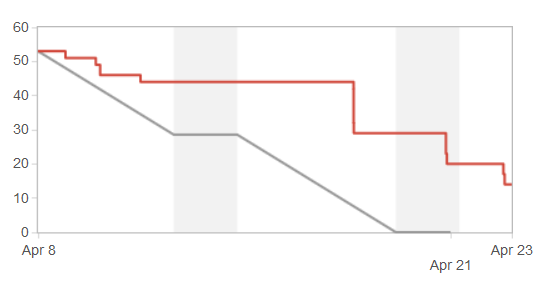
\includegraphics[scale=1]{images/graph/sprint3.png}
                    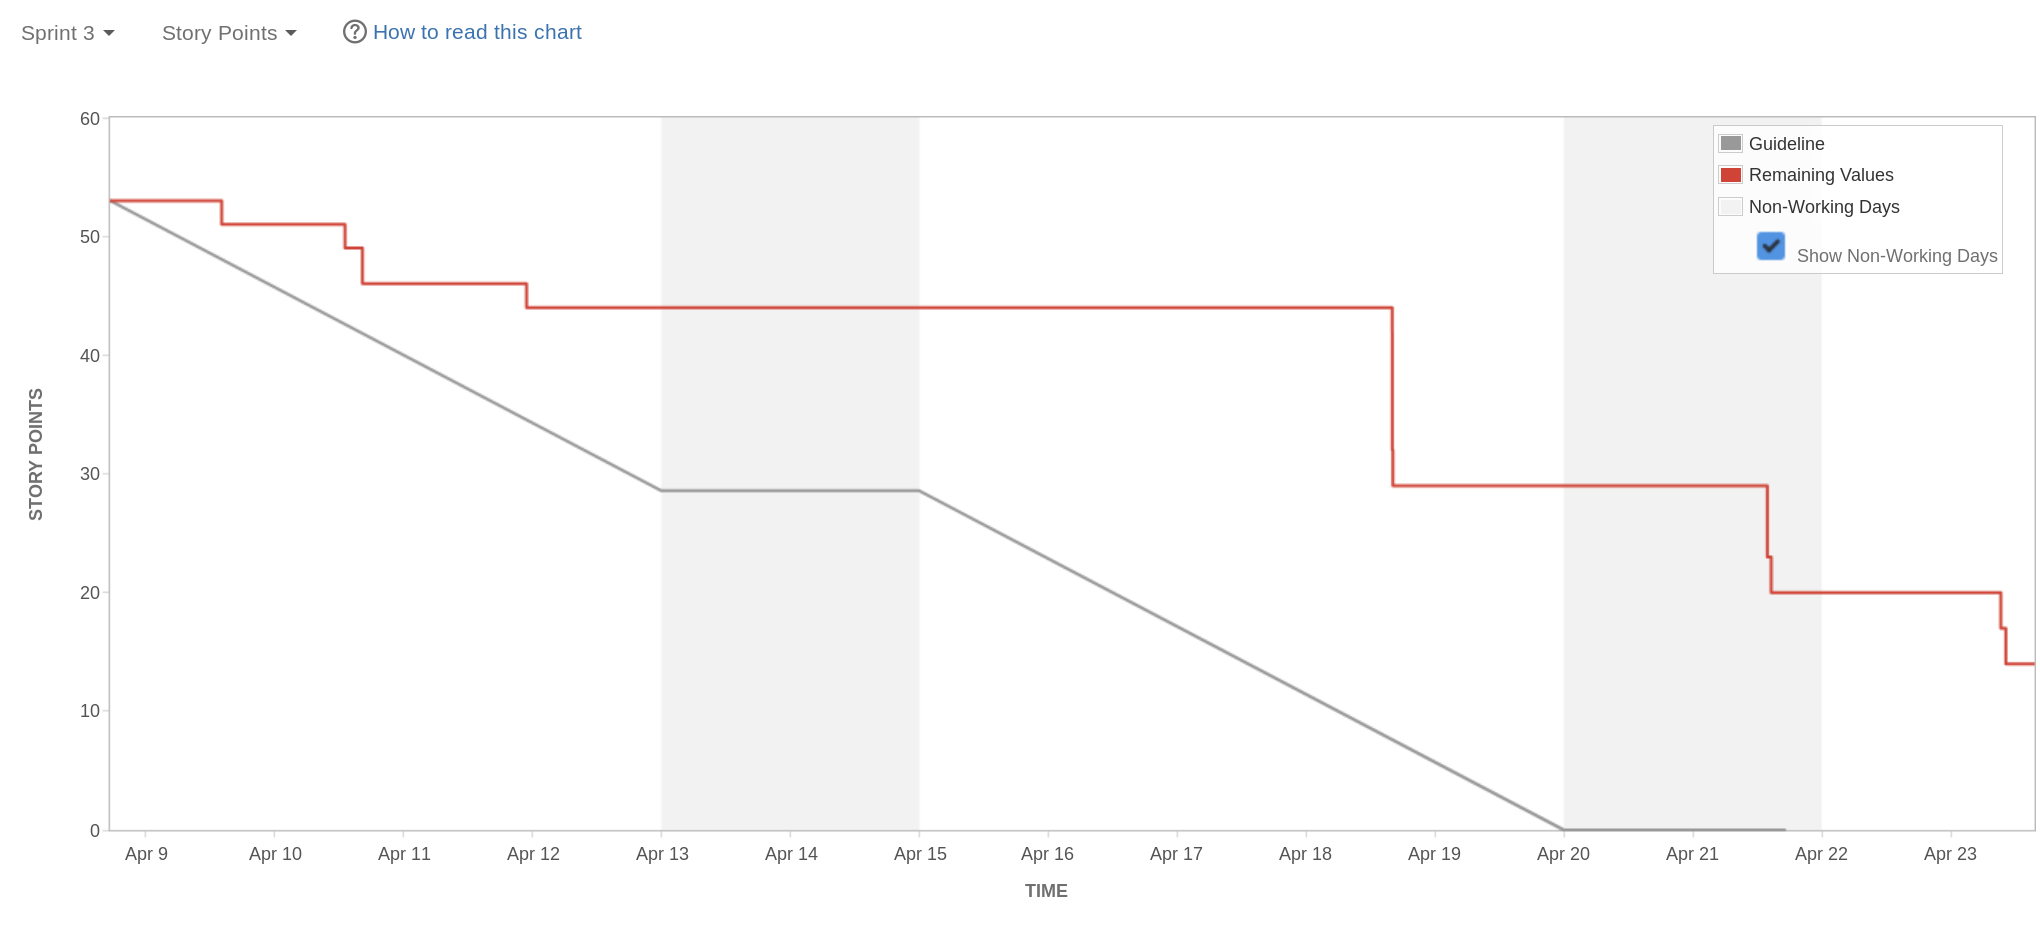
\includegraphics[scale=.25]{images/graph-new/sprint3.png}
                    \captionof{figure}{Sprint 3 - Burndown chart}
                    \label{fig:sprint3_graph}
                \end{center}
                
                \noindent Malgré cela, nous avons à nouveau fait une sur estimation du temps que nous pouvions mettre dans le développement.
                
                
            \subsubsection{Sprint 4}
                \noindent Sprint fort ressemblant au sprint précédent. Nous avons profité de la période de congé pour avancer le plus possible dans l'application. Nous avons aussi ajouté pas mal de tâches en cours de sprint car nous découvrions des bugs ou des fonctionnalités manquantes à ajouter. 
                Ceci explique en partie l'écart final dans le graphique ci-dessous.
                
                \begin{center}
                    %%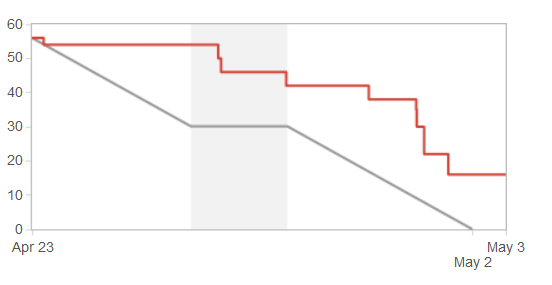
\includegraphics[scale=1]{images/graph/sprint4.png}
                    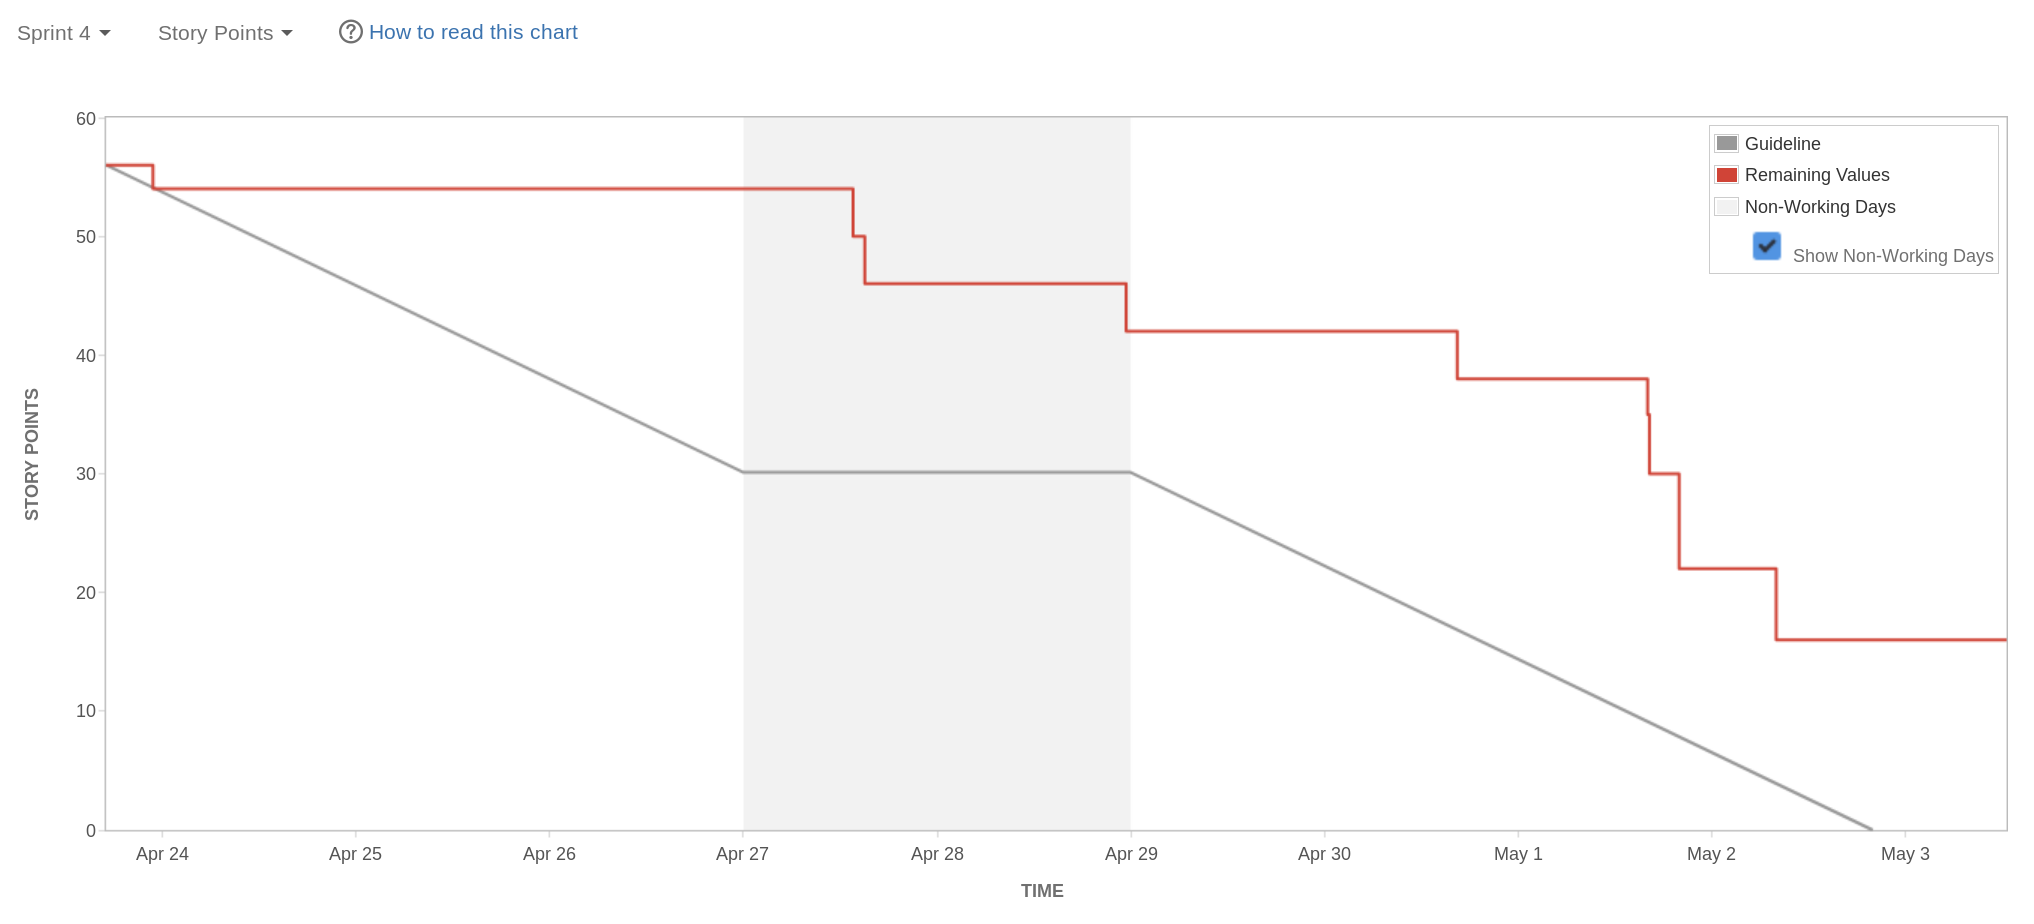
\includegraphics[scale=.25]{images/graph-new/sprint4.png}
                    \captionof{figure}{Sprint 4 - Burndown chart}
                    \label{fig:sprint4_graph}
                \end{center}
        
        
            \subsubsection{Sprint 5}
                \noindent Il s'agit du dernier sprint du projet, nous avons découvert pas mal de bugs et fonctionnalités pas assez développées mais l'ensemble de l'application était présent. Le graphique de ce sprint montre bien que des tâches ont été ajoutées en cours de sprint car la charge de travail restant monte et descend à plusieurs reprises. 
                
                \begin{center}
                    %%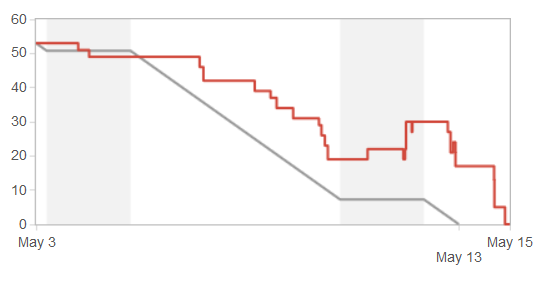
\includegraphics[scale=1]{images/graph/sprint5.png}
                    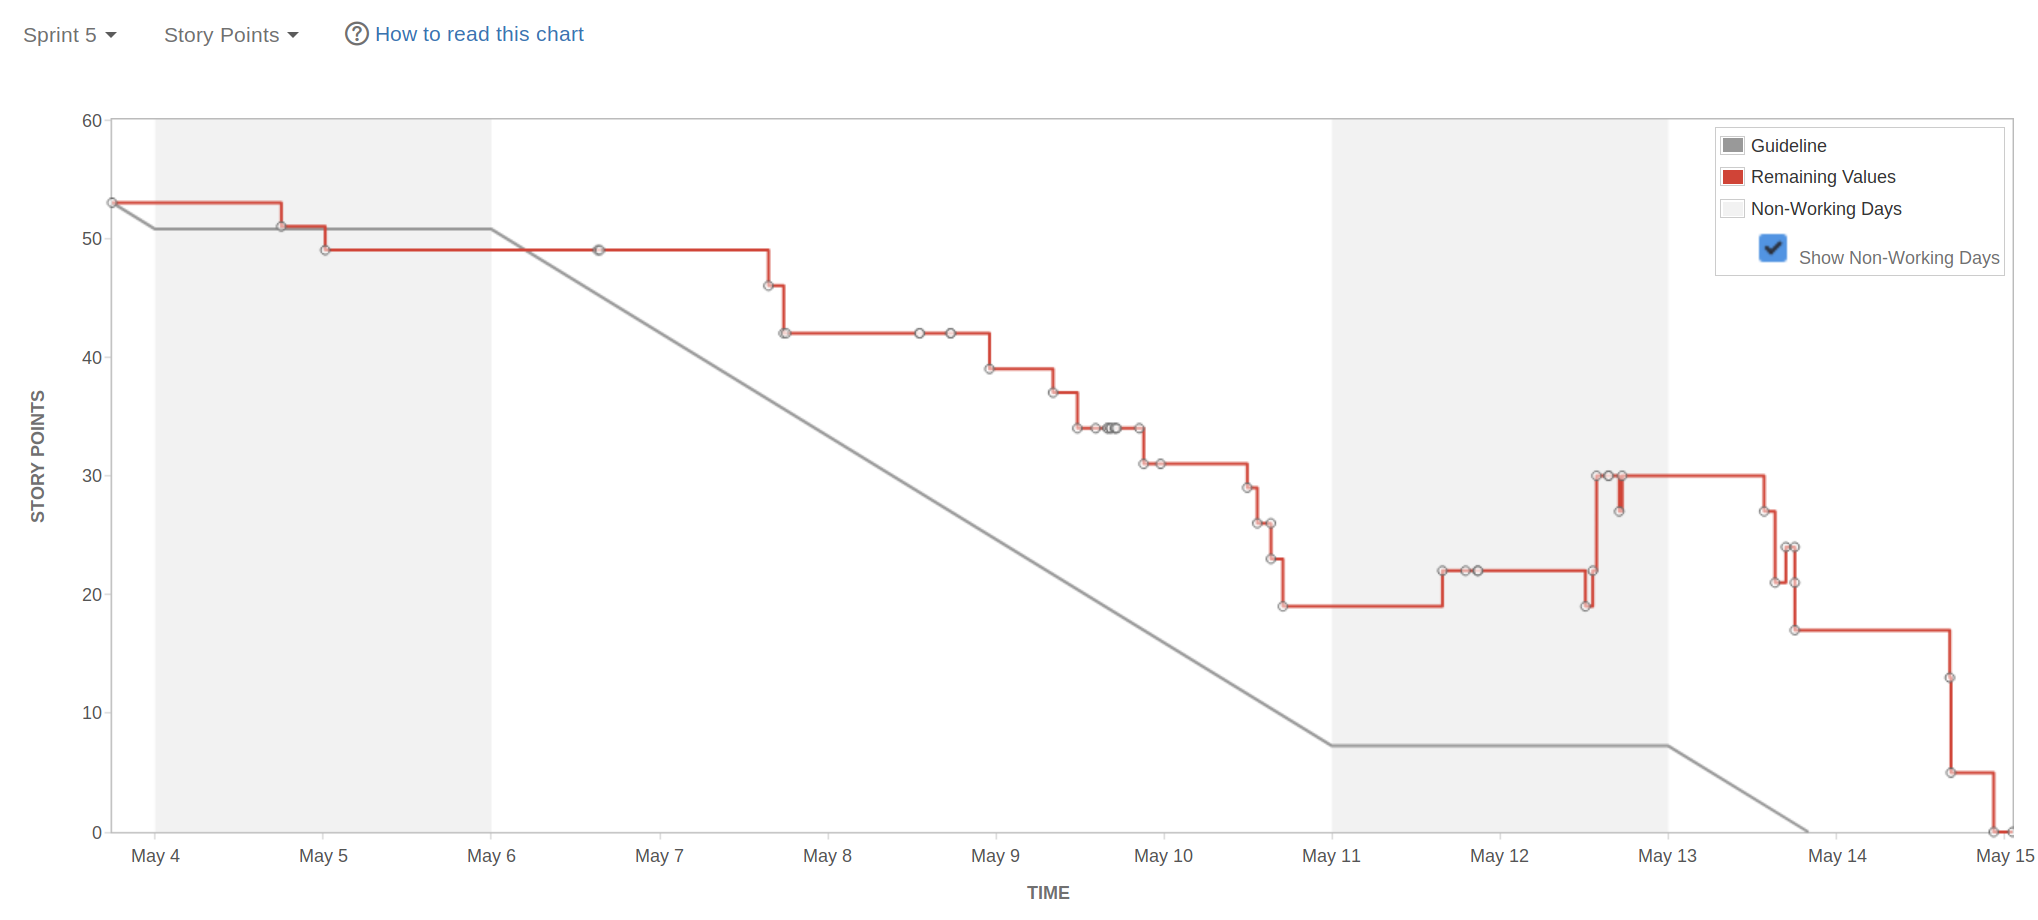
\includegraphics[scale=.25]{images/graph-new/sprint5.png}
                    \captionof{figure}{Sprint 5 - Burndown chart}
                    \label{fig:sprint5_graph}
                \end{center}
                
                
           \subsubsection{Conclusion} 
               \noindent Nous avons eu du mal au début à bien répartir les tâches avec de bonnes estimations de temps,... mais au fur et à mesure, nous avons commencé mieux nous en sortir. \\
                L'un de nos plus gros défaut dans la gestion du temps et des sprints est que nous n'avons pas fait comme montré au cours (tableaux d'emplois du temps,... pour chaque personne). Il aurait également fallu attribuer dès le début toutes les tâches de tous les sprints, et pas configurer les sprints en fin de sprint précédent. 
                
        
        \subsection{Cost Management}
    
%%%%%%%%%%%%%%%%%%%%%%%%%%%%%%%%%%%%%%%%%%%%%%%%%%%%%%%%%%%%%%%%%%%%%
    \section{Clôture du projet}
        \noindent Quand le projet a été fini et envoyé, nous nous sommes félicités et avons pris un petit peu de repos avant de nous lancer dans la préparation de la présentation orale. Après celle-ci, nous nous sommes à nouveau félicités puis nous avons rangé notre local et rendu les clés, ce qui a véritablement marqué la fin du projet.\\
        Notre projet est une réussite, nous avons rendu une application conforme aux attentes du client tout en respectant les échéances.
    
\end{document}